
\chapter{Introduction}
\label{chap:introduction}

%Kurzer Text zur Motivation für diese Arbeit; wie es zum Thema kam und wie das Ziel erreicht wurde

Introductory text -> motivation\\
- \Kp{} impact analysis\\
- solar activity analysis\\
- distance analysis\\

% Questions this work asks:\\	%Fragestellungen ausformuliert
% 	How strong is the solar-wind influence on the terrestrial magnetosphere?\\
% 	How often occur certain solar-wind ranges?\\
% 	How strong do different structure types influence the terrestrial magnetosphere?\\
% forecast:\\
% 	How can the impact strength of the solar wind be forecasted? (VBz->Kp L1-Alerts)\\
% 	How can the impact strength of CMEs be forecasted (V->Kp correlation for CMEs)?\\
% 	(How can the impact field strength of CMEs be forecasted (V->B correlation for CMEs)?)\\

% 	How does the solar wind evolve on its way from the Sun?\\
% 	How do the different structures evolve on their way from the Sun?\\
% 	What are the properties of the solar wind near the Sun?\\
% 	(Where does the solar wind get accelerated?)\\
% 	(How does the solar wind get accelerated?)\\
% 	(How is this related to the coronal heating problem?)\\

thesis goal: finding more precise relationships between parameters/quantities for being able to make better forecasts\\

%Synopsis	% Outline (chapters and their content)
This thesis merges the solar-wind analyses of its impact on the magnetosphere, its variation with solar activity, and its evolution to Earth. This work is structured as follows. In \autoref{chap:basics} the fundamentals about the Sun, its activity, solar wind, and space weather are laid. The instruments and data are described in \autoref{chap:data}. The influences on the \Kp{}~index from solar activity, solar wind, its streams, and CMEs are analyzed in autoref{chap:chapter2}. In \autoref{chap:empirical_solar_wind_model_for_the_inner_heliosphere}, which includes the published paper on the same topic (\autoref{chap:solar_wind_predictions_for_the_parker_solar_probe_orbit}), an empirical solar-wind model for the inner heliosphere is developed and used to estimate the near-Sun solar-wind environment for the planned PSP mission. \autoref{chap:summary} summarizes the results and gives an outlook for further studies. Useful equations, constants, and abbreviations are located in the \autoref{chap:physics}, \ref{chap:math}, and \ref{chap:glossary}.


\chapter{Background knowledge}
\label{chap:basics}
%COFI -- chapter outline and flow integration
This chapter summarizes the basic knowledge, which is necessary for the analyses performed in this work. First, the Sun's origin, inner structure, atmosphere and heliosphere are described. Then, the Sun's dynamics with its differential rotation and magnetic field generation are outlined. Further, the solar activity cycle is described, including the meridional flow circulation, appearance of active regions, the surface magnetic field change, and sunspot cycles. The heliospheric magnetic field is pictured from its photospheric emergence in magnetic bright points and coronal superradial expansion, through the formation of the heliospheric current sheet and the Parker spiral to the heliosheath. The solar wind and its properties, the origin of slow and fast streams, stream interaction regions, and coronal mass ejections are described. Furthermore, the space weather, the solar influence on Earth, the magnetosphere, solar wind-magnetosphere coupling, and geomagnetic indices are portrayed.
%first the existing structures, second their dynamics, last their influence on humans/their technology (space weather)


\section{The Sun}
\label{sec:solar_composition}

%%% universe
13.8~billion years ago the Big~Bang formed our universe. The energy density of our universe consists of \SI{69.1}{\percent} dark energy, \SI{25.9}{\percent} dark matter and \SI{4.9}{\percent} baryonic matter, according to calculations using the inflationary $\Lambda$CDM\footnote{$\Lambda$CDM: Lambda cold dark matter} cosmology together with the latest cosmic microwave background temperature measurements \citep{Planck2016}.
%see Planck2016 page 31 Table 4		age of universe
%see Planck2016 page 31 Table 4 and en.wikipedia.org/wiki/Lambda-CDM_model#Parameters
%energy density consists of
%dark energy $\Omega_\Lambda = 0.6911$,
%matter $\Omega_\text{m} = 0.3089$,
%dark matter $\Omega_\text{c} = 0.2589$ and
%baryonic matter $\Omega_\text{b} = 0.0486$
After a few minutes the primordial nucleosynthesis left the universe in a state where the baryonic matter was composed of \SI{75.33}{\percent}\footnote{Percentages by mass.} hydrogen, \SI{24.67}{\percent} helium and traces of deuterium, tritium and lithium \citep{Planck2016}.
%see Planck2016 page 47 Eq. 73

%%% star formation
Over millions of years this gas cooled down and gravitationally accreted into molecular clouds and formed stars. The first generations of stars (Population~III) fused this gas to heavier elements (metals) and supernovae distributed them into space as a foundation for the formation of new stars of low and high metallicity (Population~II and I). Likewise, supernovae of these stars constantly enriched the interstellar medium with metals. Now, the interstellar medium in the Milky~Way consists of about \SI{32}{\percent} helium and traces of other metals \citep{Danziger1970}.\\
%In 20XX the Voyager~? probe measured a density of about ...\SI{0}{\per\cm\cubed} right outside of the heliopause (cite?).\\

%%% solar interior
Our Sun, a metal-rich Population~I yellow dwarf star, emerged 4.6~billion years ago \citep{Bahcall1995} from an accretion disk, formed by a collapsing rotating cloud. The compression within its center resulted in high temperatures, which initiated the fusion of hydrogen to helium (primarily pp~chain reaction). The fusion reactions produce huge amounts of energy and heat the solar center to a temperature of 15.7~million~kelvins \citep{Christensen-Dalsgaard1996}. The generated energy is transported through the solar body to its surface and eventually into space.
The core region extends to about 0.25~solar radii (\Rsun), where the declining temperature becomes insufficient for fusion reactions. The energy transport is dominated by thermal radiation until, because of declining ionization and density, at 0.71\,\Rsun{} up to the surface convective motion takes over \citep{Christensen-Dalsgaard1991}. %0.7: http://adsabs.harvard.edu/abs/1991ApJ...378..413C
%Dalsgaard Model S: http://astro.phys.au.dk/~jcd/solar_models/
%core radius (cite?)

%%% photoshere + sunspots
The temperature at this transition region (tachocline) is about 2~million~kelvins and decreases up to the solar surface to between \SIrange{4400}{6600}{\K} (cite?). Here at the photosphere, the energy is radiated away with an effective black body temperature of \SI{5772}{\K} \citep{Mamajek2015}, classifying the Sun as a spectral type G2V star.
At this surface layer granules, the tops of convection cells, and temporary sunspots are visible. Strong magnetic flux inhibits the convection at sunspots, leading to lower temperature and brightness (for more details on sunspots see the next \autoref{sec:solar_dynamics}). \autoref{fig:sun_interior_HMIIC} illustrates these photospheric features along with the inner solar structure.\\
\begin{figure}[htb]
	%\centering
	\fcapside[\FBwidth]{
		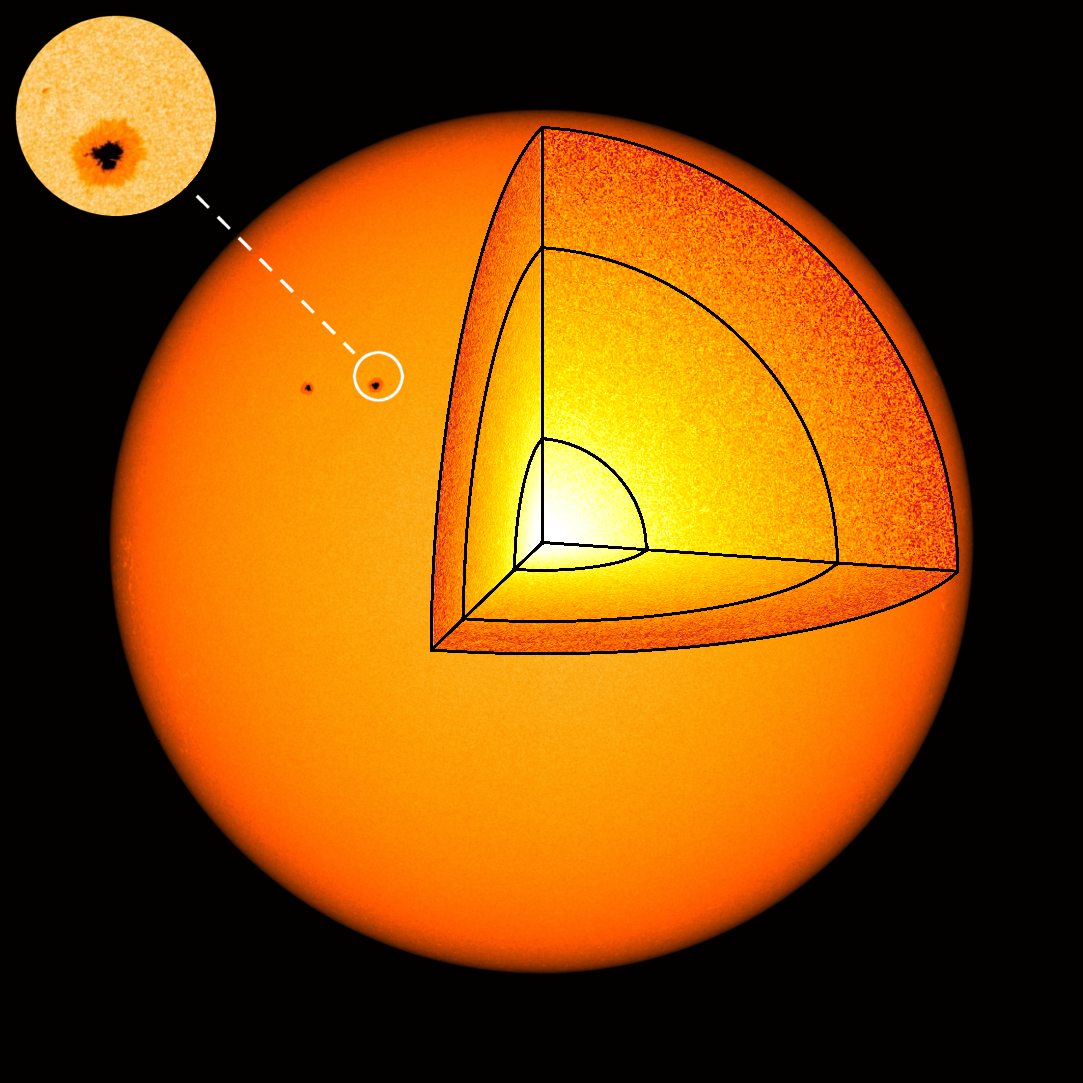
\includegraphics[width=0.6\textwidth]{images/own_figures/sun_interior_HMIIC.png}
	}{
		\caption{Image of the photosphere together with a schema of the solar interior structure. The inset shows the granular surface with a sunspot. The figure is based on a SDO/HMI continuum image from 20~March~2016, credit: NASA/SDO and the AIA, EVE and HMI science teams.}
		\label{fig:sun_interior_HMIIC}
	}
\end{figure}

%%% chromosphere + corona + CMEs
Above the photosphere at the base of the chromosphere, the temperature declines to its solar minimum of \SI{3800}{\K} until it raises to \numrange{2}{3}~million~kelvins in the corona \citep{Billings1959,Liebenberg1975}. Up to now it is not fully understood why the corona is so much hotter than the underlying chromosphere -- this question is known as the coronal heating problem (cite?!). The generally considered energy transfer mechanisms are magnetic reconnections, wave heating and type~II spicules or a combination of these (cite?).

The chromosphere is a \SI{2000}{\km} thick region, whose features -- numerous spicules, filaments, and prominences -- can reach far into the corona. They consist of chromospheric material channeled by the solar magnetic field, which is enveloped by a thin transition region where the temperature jumps up from ?\SIrange{20000}{35000}{\K} to coronal temperatures (cite?). Reconnection of magnetic field lines can result in the eruption of filaments into the corona and beyond, termed coronal mass ejections (CMEs) (see also Section~XX...). Details of chromospheric features are shown in \autoref{fig:sun_atmosphere}.

%%% coronal holes
The Sun's atmosphere is dominated by the varying small- and large-scale solar magnetic field configuration. There are regions where the magnetic field lines arc back to the surface and regions with open field lines. In the latter areas the coronal plasma can -- guided by the field -- escape into space. Thus these coronal areas are less dense, cooler and therefore appear darker in extreme ultraviolet (EUV) and are called coronal holes (more in Section~XX...). In \autoref{fig:sun_atmosphere} a coronal hole is visible at the solar south pole.
\begin{figure}[htb]
	%\centering
	\fcapside[\FBwidth]{
		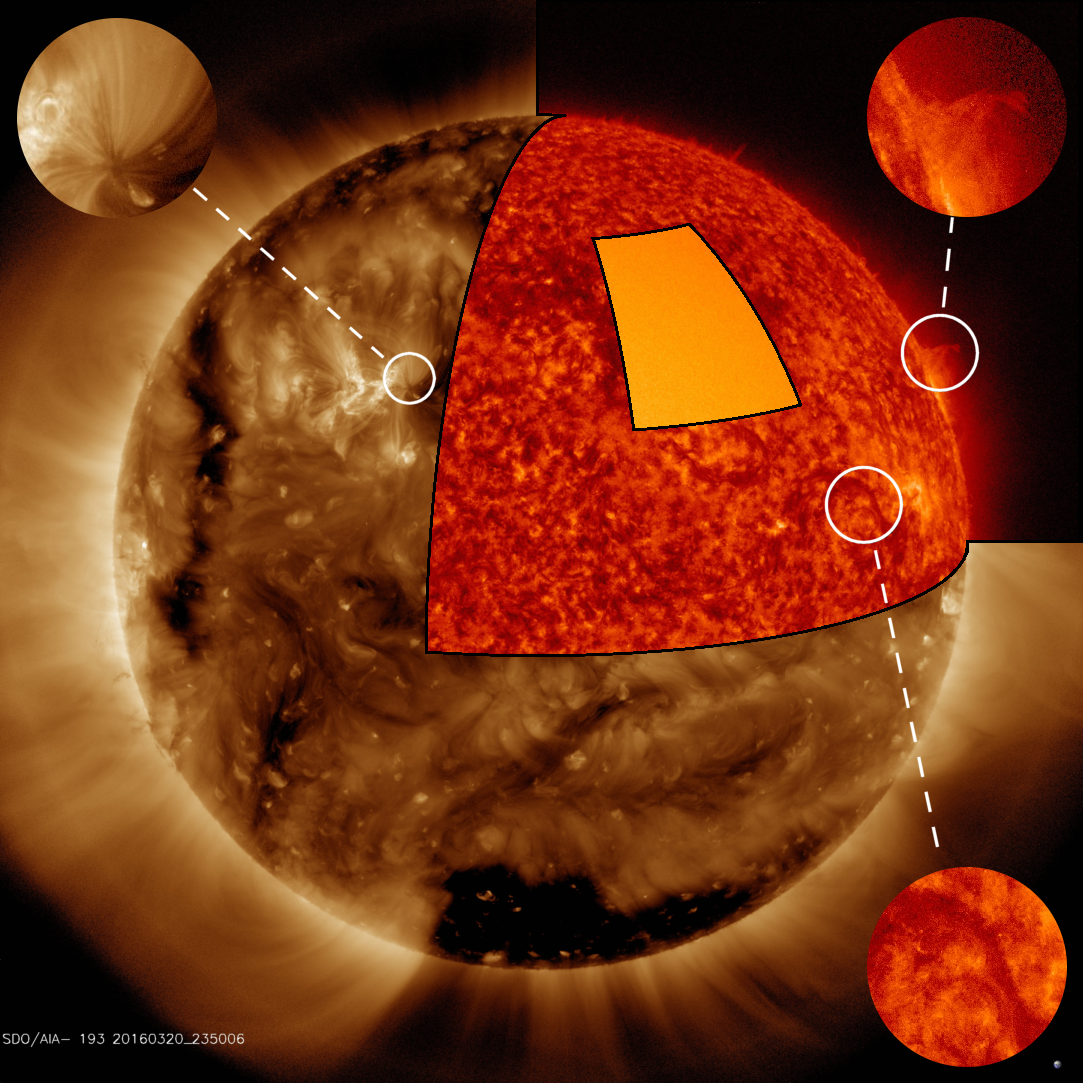
\includegraphics[width=0.6\textwidth]{images/own_figures/sun_atmosphere.png}
	}{
		\caption{Composite image of the solar atmosphere and some of its features. Corona, chromosphere and photosphere are seen in wavelengths of \SI{193}{\angstrom}, \SI{304}{\angstrom} and continu\-um. Chromospheric spicules are visible on the northern limb. The enlargements on the right show a prominence and a filament. The dark region at the south pole is a coronal hole. The left inset shows details of the active region belonging to the sunspots in \autoref{fig:sun_interior_HMIIC}. The figure is based on SDO/AIA images from 20~March~2016, credit: NASA/SDO and the AIA, EVE and HMI science teams.}
		\label{fig:sun_atmosphere}
	}
\end{figure}

%%% corona
From Earth, the faint corona and chromosphere can only be observed during eclipses, because of the brightness of the solar disk. There are three effects contributing to the visibility of the corona: photon scattering off free electrons and dust particles, and ion spectral emission lines (termed K-, F- and E"~corona).
% the so-called K-, F- and E"~corona (K kontinuierlich, F Fraunhofer, E emission).\\
% K-corona: photon scattering off free electrons --> coronagraphs\\
% F-corona: photon scattering off dust particles; contains Fraunhofer absorption lines; expands in ecliptic as zodiacal light --> coronagraphs\\
% E-corona: ion spectral emission lines; reveals coronal composition --> images\\
The image of a solar eclipse reveals the coronal plasma, shaped by the magnetic field, and features of the red chromosphere, pictured in \autoref{fig:Tse2008_500_mo1}.\\
\begin{figure}[htb]
	%\centering
	\fcapside[\FBwidth]{
		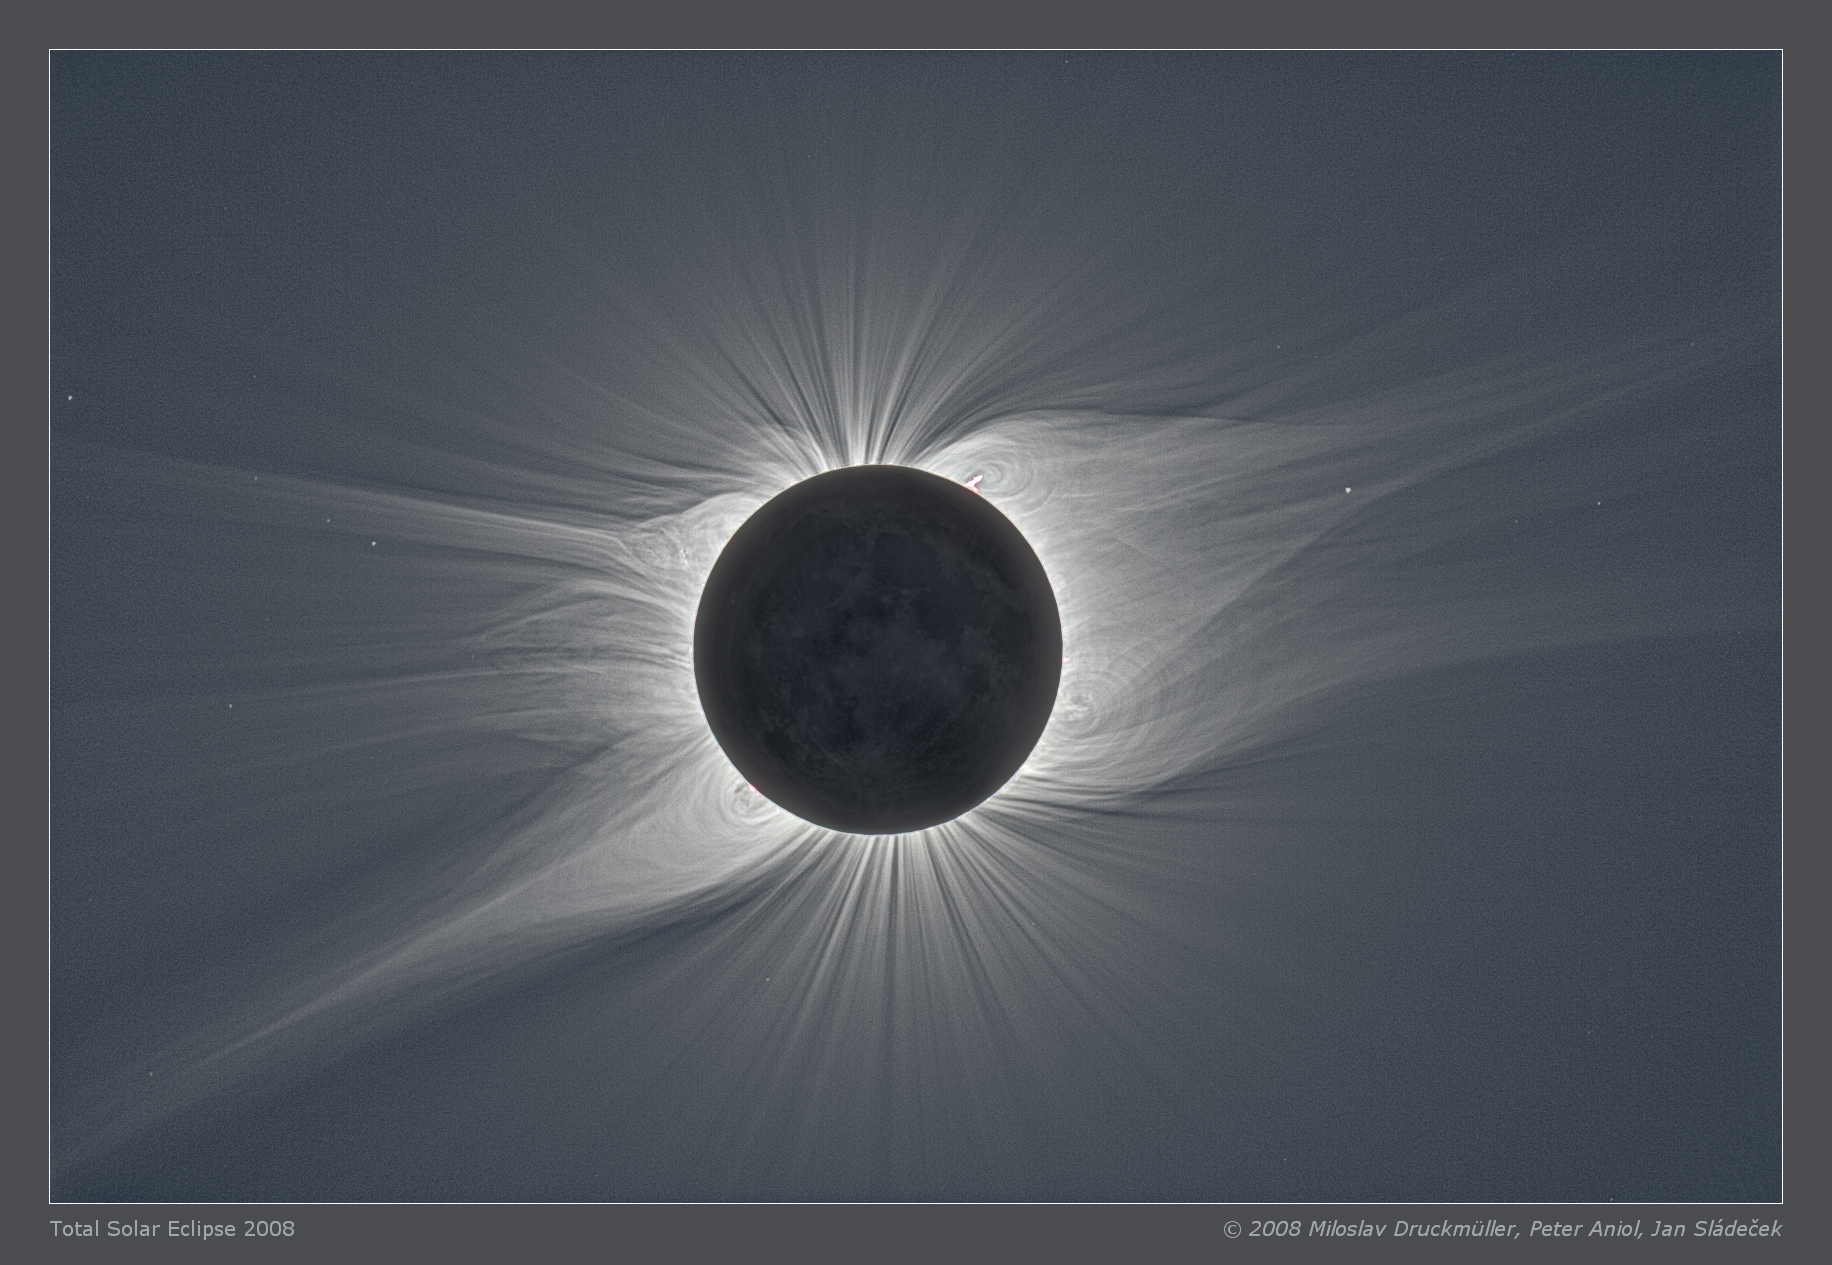
\includegraphics[width=0.6\textwidth]{images/Tse2008_500_mo1.png}
	}{
		\caption{Total solar eclipse image of the inner corona up to 5~solar radii. The picture was taken in Mongolia, 1~August~2008 and is processed from multiple images. The magnetic field's dipole structure and the equatorial streamer belt, typical for a quiet Sun in cycle minimum, are visible. Credit: \href{http://www.zam.fme.vutbr.cz/~druck/Eclipse/}{Miloslav Druckmüller, Peter Aniol, Jan Sládeček}, 2008, reproduced with permission.}
		\label{fig:Tse2008_500_mo1}
	}
\end{figure}
%figure source: http://www.zam.fme.vutbr.cz/~druck/Eclipse/Ecl2008m/Tse2008_500_mo1/Hr/Tse2008_500_mo1.png

%%% solar-wind + heliosphere
Due to the high coronal temperatures, plasma escapes from the solar gravitational field \citep{Parker1958} with velocities of \SIrange{200}{800}{\km\per\s}. Its acceleration is linked to the coronal heating, however the exact location and process remain an open question (cite?). The magnetic field becomes too weak to guide the coronal plasma at a distance of a few solar radii. From this source surface, the solar wind flows radially outward into space until it reaches the termination shock. Eventually it collides with the local interstellar medium, creating the boundary of the heliosphere, the heliopause, which is expected to be a bubble of either teardrop or croissant shape (and may be led by a bow shock), caused by the Sun's relative velocity of \SI{23}{\km\per\s} to the local interstellar medium \citep{Owens2013, Opher2015}. Measurements of the Voyager~1 and 2 spacecraft indicate their passage of the termination shock at about \SI{94}{\au} and \SI{84}{\au}, entering the heliosheath region \citep{Owens2013}. \citet{Gurnett2013} report that in 2012 Voyager~1 actually crossed the heliopause into interstellar space at a solar distance of \SI{121}{\au}. \autoref{fig:Owens2013_Heliosphere_screenshot} illustrates the heliosphere and its surrounding flow structure.
\begin{figure}[htb]
	%\centering
	\fcapside[\FBwidth]{
		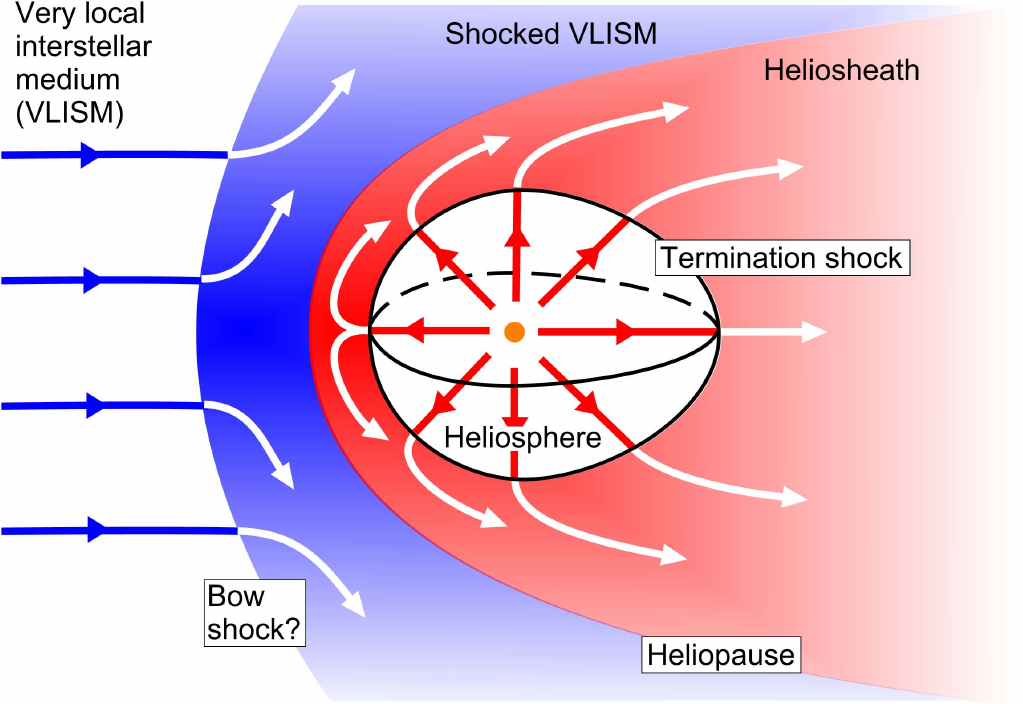
\includegraphics[width=0.6\textwidth]{images/Owens2013_Heliosphere_screenshot.png}
	}{
		\caption{Schema of the heliosphere and its surrounding flow structure. The heliosphere is formed by the interaction of the solar wind with the local interstellar medium at the heliopause. Credit: \citet[][Fig.~9]{Owens2013}, licensed under \href{https://creativecommons.org/licenses/by-nc/3.0/de/}{CC BY-NC 3.0 DE}.}
		\label{fig:Owens2013_Heliosphere_screenshot}
	}
\end{figure}
% contacted for permission...
%Owens2013 figure permission request: open access article

%%% solar-wind influence + space weather
On its way outwards through the solar system, the solar wind -- carrying the solar magnetic field -- interacts with the planets, their magnetic fields and other solar system bodies. These interactions have various effects, for instance disturbances in planetary magnetic fields with appearance of aurorae and enhanced radiation, atmospheric losses and stripping of cometary tails. Some of these effects can have disruptive consequences for humans and their technology. The topic of space weather effects is further addressed in \autoref{sec:space_weather}. The magnitude of these effects depends highly on spatial and temporal variations in the solar wind, which are rooted in the dynamics of the solar magnetic field.

%%%%%%%%%%%%%%%%%%%%%%%%%%%%%
%\section{Stars/Beginning}
% introduction leading to stars; beginning from universe/big bang\\
% gravitational contraction of rotating nebula\\
% -> fusion burning; energy production\\
% In its core it fuses hydrogen to helium; 15.7~million~K; inner 25~\%\\
% energy transport -> radiation zone; up to 70~\%\\
% tachocline ~2~million~K\\
% energy transport by convection -> convection zone; up to surface\\
% convective granulation\\
% photoshere 4400--6600~K, effective black body temperature 5777~K; spectral class\\
% (herzsprung russell diagram)\\
% chromosphere... (solar atmosphere figure)\\
% transition region\\
%corona 1--3~million~K temperature (coronal heating problem)\\
% coronal holes: open magnetic field lines, solar wind\\
% heliosphere, shock with interstellar medium (ISM); Voyager\\

%%%%%%%%%%%%%%%%%%%%%%%%%%%%%
%big bang
%to formation of stars
%to ISM in our galaxy
%to formation of Sun
%Sun's inner structure (energy production and transport)
%its surface (radiation, spectral class)
%its outer structure (chromosphere, corona, solar wind, heliosphere)
%its heliosphere (termination shock with ISM, Voyager measurements)
%%%%%%%%%%%%%%%%%%%%%%%%%%%%%


\section{Solar dynamo}
\label{sec:solar_dynamics}
%%% differential rotation + solar magnetic field origin
The spin conservation of the contracting molecular cloud led to a rotation of the Sun with a current average period of about 25~days. The radial convective motion within the solar interior above the tachocline leads to a transport of momentum away from the rotation axis and therefore to a slower polar and faster equatorial rotation in the convection zone \citep{Miesch2005}. This differential rotation is visible on the surface and was first discovered from sunspot observations. %in 1630 https://en.wikipedia.org/wiki/Solar_rotation
With a rotation period of about 34~days the poles have a lag of almost 9~days (for further information on solar rotation see appendix \autoref{sec:solar_surface_differential_rotation}). The differential rotation in the solar interior can be inferred from helioseismological observations, see \autoref{fig:Miesch2005_fig1a_interior_diff_rot}.
\begin{figure}[htb]
	\begin{floatrow}
		\ffigbox{	%[\FBwidth][]{
			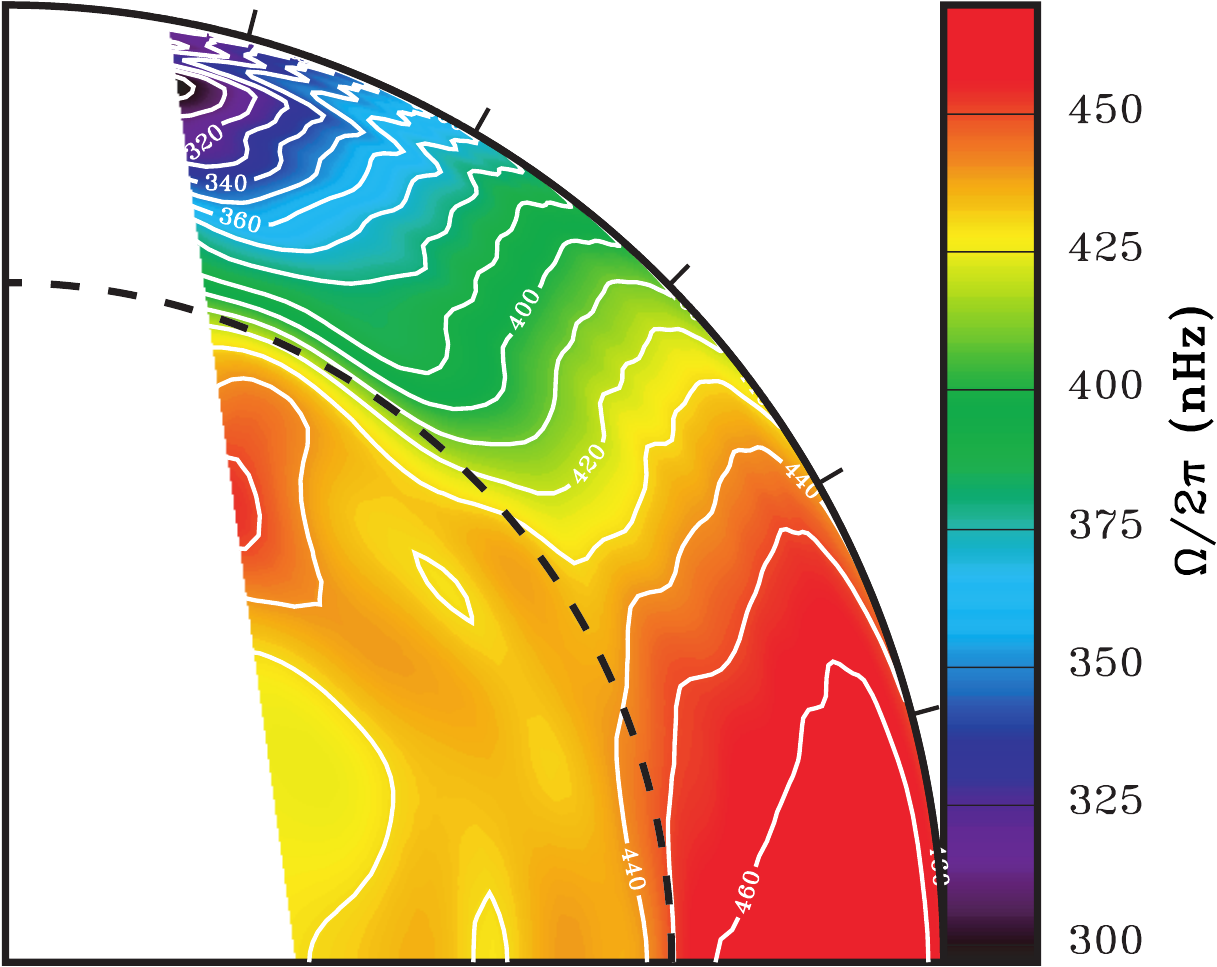
\includegraphics[width=0.5\textwidth]{images/Miesch2005_fig1a_interior_diff_rot.png}
		}{
			\caption{Angular rotation velocity in the solar interior. The radiation zone has a nearly solid rotation. Above the tachocline (dashed line) begins the differential rotation of the convection zone. The angular velocity is inferred from helioseismology via observations from the Michelson Doppler Imager (MDI) at the Solar and Heliospheric Observatory (SOHO) spacecraft. Credit: \citet[][Fig.~3]{Thompson2003}, reproduced with permission, \textcopyright~Annual~Reviews.}
			%(\citet[Fig.~1\,a]{Miesch2005}; based on \citet[Fig.~3]{Thompson2003})
			\label{fig:Miesch2005_fig1a_interior_diff_rot}
			%Thompson2003 permission request: permission not required
		}
		\ffigbox{
			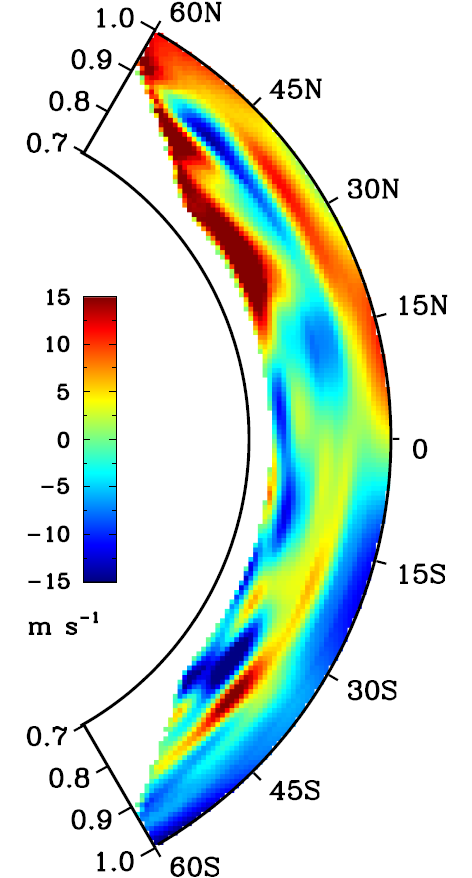
\includegraphics[width=0.28\textwidth]{images/Zhao2013_meridional_flow.png}
		}{
			\caption{Meridional flow velocity profile in part of the convection zone. Positive values are directed towards north. The velocity is inferred from helioseismology via observations from the Helioseismic Magnetic Imager (HMI) at the Solar Dynamics Observatory (SDO) spacecraft. Credit: \citet[][Fig.~4,\,panel~a]{Zhao2013}, reproduced with permission, \textcopyright~AAS.}
			\label{fig:Zhao2013_meridional_flow}
			%Zhao2013 permission request: permission granted.
		}
	\end{floatrow}
\end{figure}
%Angular velocity profile in the solar interior inferred from helioseismology (after Thompson et al., 2003). In panel (a), a 2D (latitude-radius) rotational inversion is shown based on the subtractive optimally localized averaging (SOLA) technique. All inversions are based on data from the Michelson Doppler Imager (MDI) instrument aboard the SOHO spacecraft, averaged over 144 days. Inversions become unreliable close to the rotation axis, represented by white areas in panel (a). Note also that global modes are only sensitive to the rotation component which is symmetric about the equator (courtesy M.J. Thompson \& J. Christensen-Dalsgaard).

%%% magnetic field dynamo mechanism
Turbulent plasma motions from convective flows in the convection zone generate and carry magnetic flux. The large rotational shear at the tachocline stretches and amplifies the disorganized magnetic fields ($\omega$-effect) to strong coherent toroidal flux with intensities of the order \SIrange{1}{10}{\tesla}. These toroidal fields, generated near the bottom of the convection zone, can be stored in a deep magnetic layer located in the stably stratified region below the convection zone \citep{Ossendrijver2003}. The stronger flux ropes become buoyant and raise to the surface. The Coriolis force twists them systematically, the twist is stronger at higher latitudes (Joy's law), on their way through the convection zone ($\alpha$-effect). They emerge then on the photosphere as bipolar active regions -- the stronger ones forming pairs of sunspots, see \autoref{fig:bipolar_region_HMIB_HMIIF}.
\begin{figure}[htb]
	\centering
	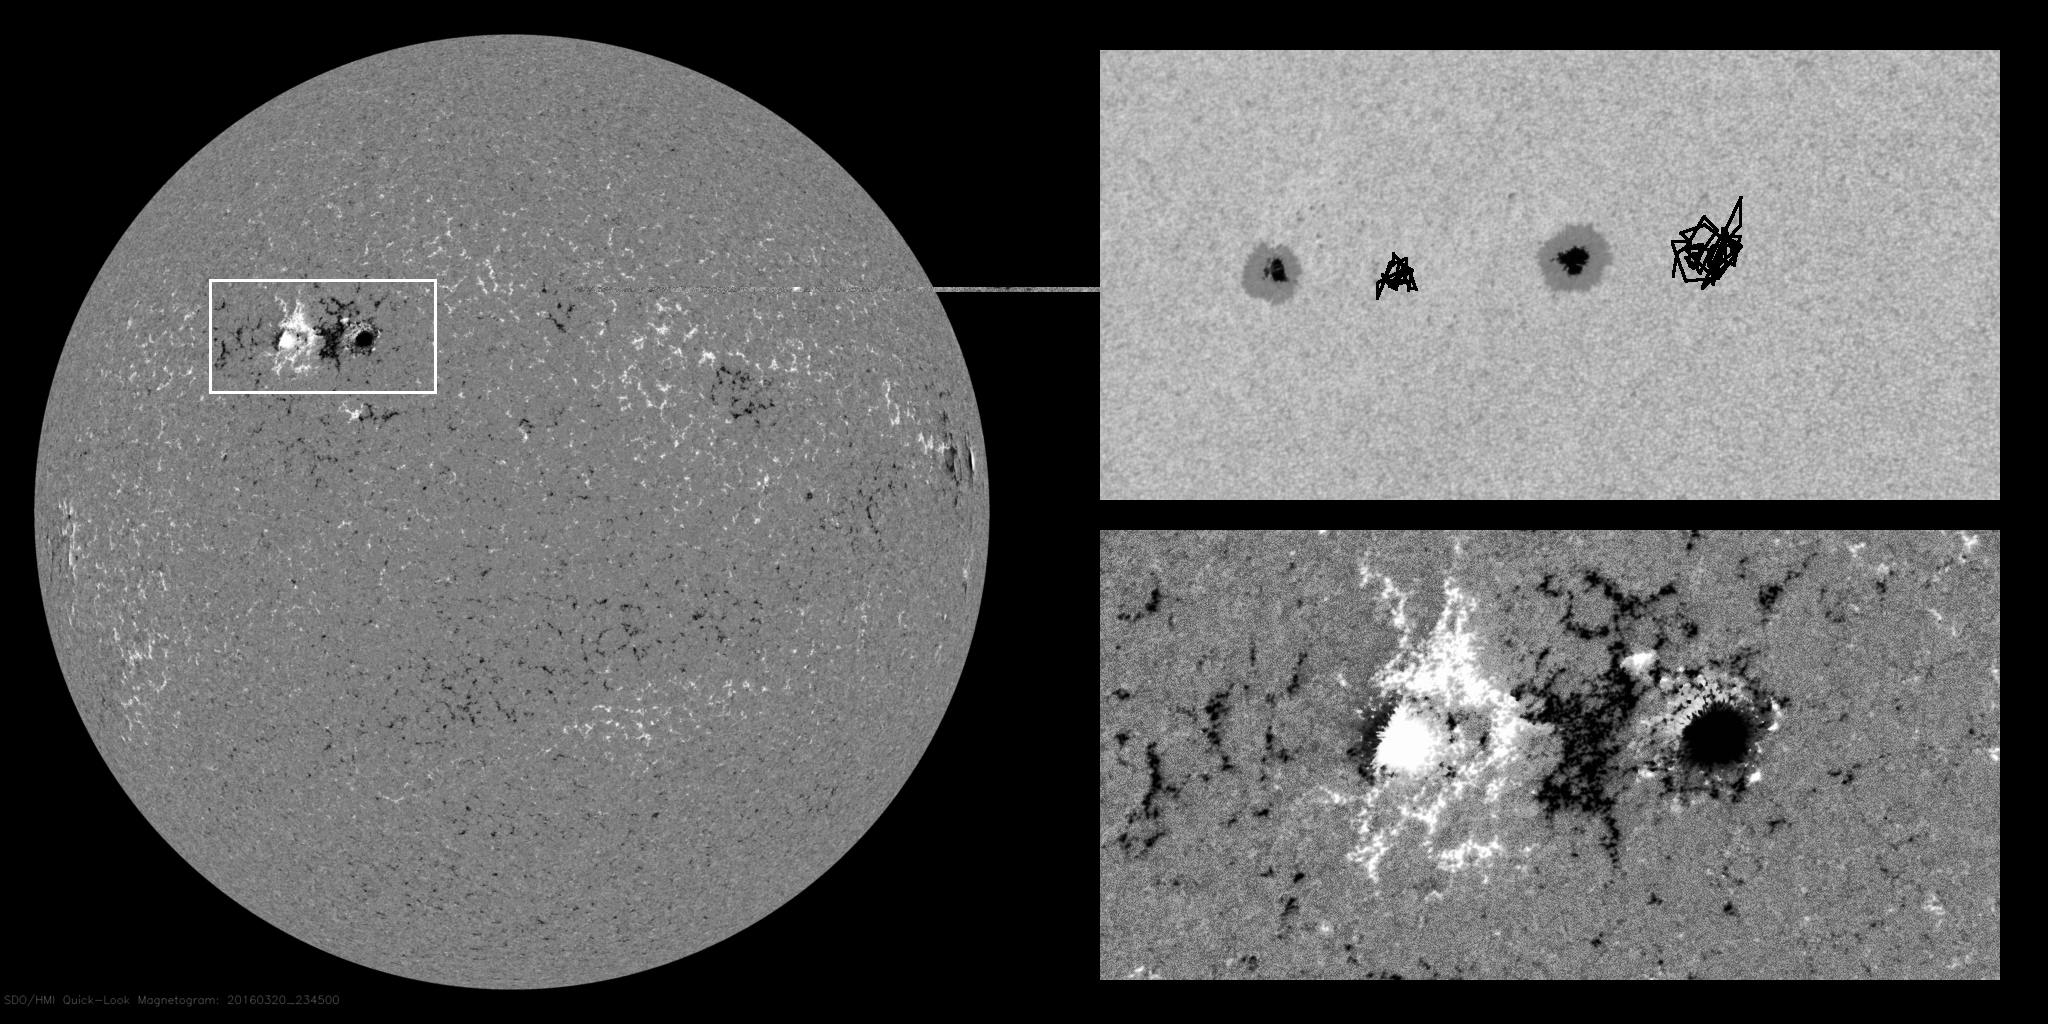
\includegraphics[width=\textwidth]{images/own_figures/bipolar_region_HMIB_HMIIF.png}
	\caption{Continuum image of both sunspots from \autoref{fig:sun_interior_HMIIC}, magnetogram from the same region and from the whole solar disk. The magnetogram shows the polarity of the line-of-sight magnetic field component at the photosphere (black/white: inward/outward polarity). The highly concentrated magnetic flux at the sunspots is clearly visible in the magnetogram as well as the extended bipolar magnetic field structure of the whole active region. The solar disk is scaled to the same size as in \autoref{fig:sun_interior_HMIIC}. The figure is based on SDO/HMI continuum and magnetogram images from 20~March~2016, credit: NASA/SDO and the AIA, EVE and HMI science teams.}
	\label{fig:bipolar_region_HMIB_HMIIF}
\end{figure}
% HMI is a vector magnetogram, but the public sources say that the magnetogram shows a line-of-sight magnetic field.
Turbulent convective diffusion of this surface flux contributes to the build-up of poloidal fields. Their resulting polarity is opposite to the prevailing global field, due to the directional way the rotational shear at the tachocline and the Coriolis force in the convection zone act. Fluctuating motions further amplify the mean fields in these processes. This solar $\alpha$-$\omega$-dynamo is thought to create the major part of the solar magnetic field. Still, with regard to the magnetic field's high variability, the long-term mean fields are governed by intermittent localized structures, that is, active regions, filaments and coronal loops \citep{Miesch2005}.	%Miesch2005 p.~18 + p.~31

the $\alpha$-$\omega$-dynamo, see \autoref{fig:EOSFIG2_modified}\\
\begin{figure}[htb]
	%\centering
	\fcapside[\FBwidth]{
		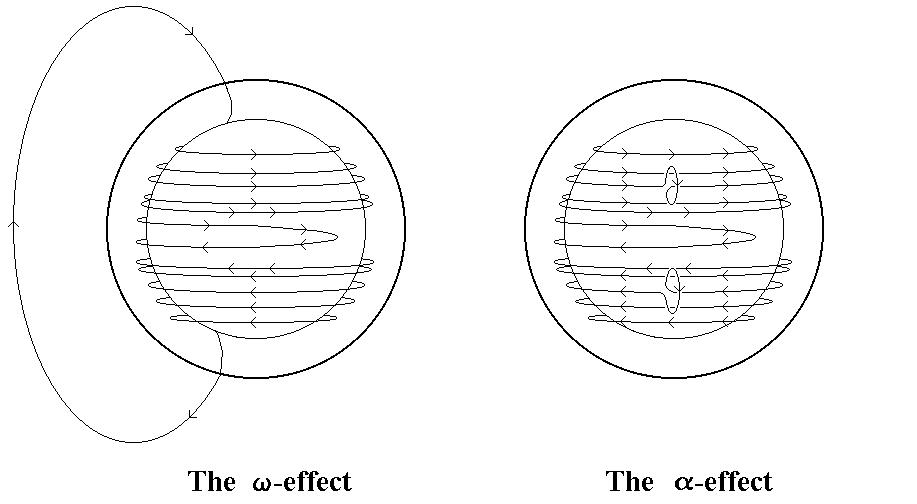
\includegraphics[width=0.5\textwidth]{images/EOSFIG2_modified.png}
	}{
		\caption{Schemata of the $\omega$ and the $\alpha$-effects. figure really necessary? get permission...}
		\label{fig:EOSFIG2_modified}
	}
\end{figure}
%http://certificate.ulo.ucl.ac.uk/modules/year_one/NASA_MSFC/solar_physics/dynamo.htm
%https://solarscience.msfc.nasa.gov/images/EOSFIG2.GIF

% switching between states of strong poloidal and toroidal field\\
% poloidal field + diff. rot. => toroidal field ($\Omega$-effect)\\
% the solar dynamo: (toroidal to poloidal field)\\
% - turbulent plasma motions from convective flows generate disorganized magnetic fields\\
% - differential shear at tachocline amplifies fields to strong coherent toroidal flux ($\Omega$-effect); magnetic layer located at the base of the convection zone\\
% - stronger flux ropes raise to surface (buoyantly)\\
% - Coriolis force twists them systematically, stronger at higher latitudes\\
% - twisted tubes emerge on the surface as bipolar active regions\\
% - amplification of mean fields by fluctuating motions ($\alpha$-effect) and turbulent diffusion create large-scale poloidal field\\


\section{Solar activity cycle}
\label{sec:solar_activity_cycle}
%%% convection cycle + solar surface magnetic field + solar cycle
Helioseismic measurements reveal that the large-scale convective flow is agglomerated into large convection cells with slow meridional flows of a few \si{\m\per\s}, see \autoref{fig:Zhao2013_meridional_flow}. A poleward subsurface flow and equatorward backflow beneath with a further poleward flow below are detected within each hemisphere, comprising a stacked double-cell profile. The meridional circulation flow speed has a major influence on the average 22-year period of the emerging magnetic flux at the solar surface. This period varies and is influenced by the stochastic emergence rate and tilts of active regions and the diffusion from random convective motions \citep{Hathaway2016}. Within one period, the surface magnetic field configuration changes from a dipole structure to a reversed dipole structure with opposite polarity, thus the transition time from one dipole state to the next lasts about 11~years, this period is termed solar cycle.
%http://www.solarcyclescience.com/forum/viewforum.php?f=9

%%% butterfly pattern
In the transition phase, magnetic flux emerges in belts above and below the solar equator, manifesting as bipolar active regions with sunspots, resulting in a toroidal/multipolar structured magnetic field. Sunspots appear at about \SI{+-20}{\degree} latitude at the beginning of a cycle, this shifts towards lower latitudes at the end of a cycle. Thus the plot of sunspots over latitude and time reveals a butterfly pattern \citep{Maunder1904}. This butterfly pattern appears in surface radial magnetic field observations as well, see \autoref{fig:Hathaway_magbfly}.
\begin{figure}[htb]
	\centering
	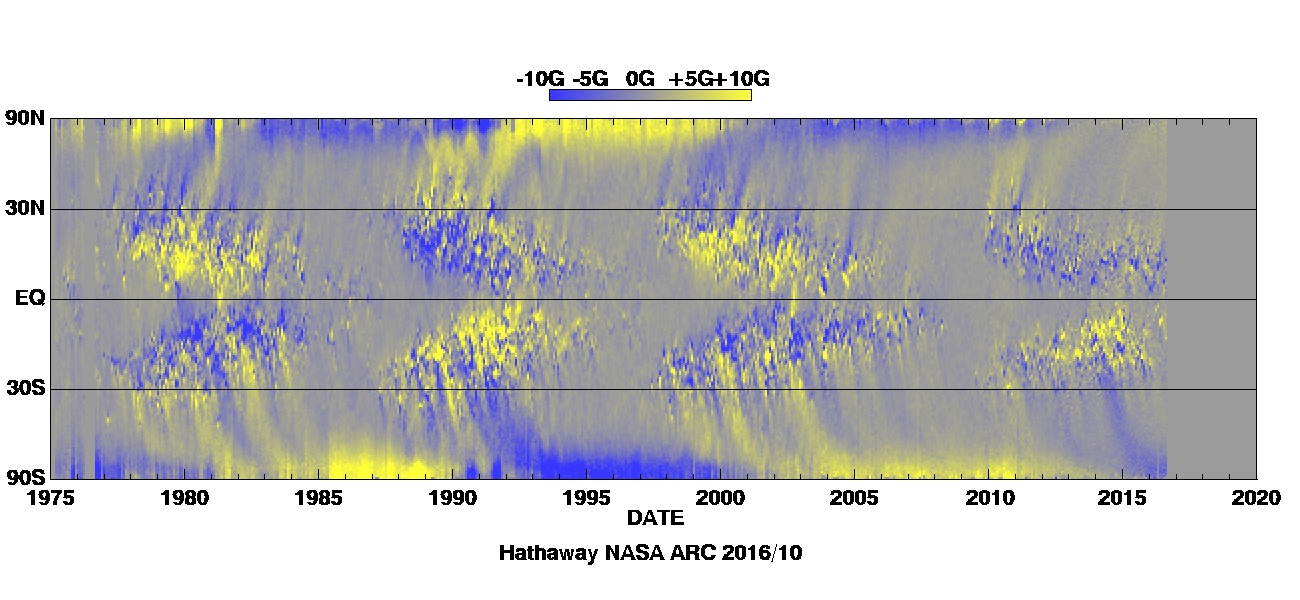
\includegraphics[width=\textwidth]{images/Hathaway_magbfly_201610.jpg}
	\caption{Magnetic butterfly diagram of the synoptic radial magnetic field on the solar surface. Yellow represents an outward directed magnetic field (positive), blue inward (negative). The data is obtained from instruments on Kitt~Peak National Observatory and from the MDI at the SOHO spacecraft. Credit: David~Hathaway, NASA Marshall Space Flight Center \citep[updated version of][Fig.~17]{Hathaway2015}. Update this figure before printing!}
	\label{fig:Hathaway_magbfly}
\end{figure}
%Hathaway 2015 permission request: open access article
%figure source:	http://solarscience.msfc.nasa.gov/images/magbfly.jpg
The leading polarity of bipolar regions is opposite in both hemispheres and the leading polarity changes with each cycle (Hale's polarity law). The emerging flux is carried by the slow meridional surface flow poleward, canceling the current dominating polar field polarity and eventually resulting in the polar field switch \citep{Hathaway2015}.

%%% sunspot number
Since regions of strong magnetic flux are visible as sunspots on the photosphere, they were known well before the common era by greek and chinese scholars \citep{Vaquero2007,Clark1978}. %greek sunspot observation: http://adsabs.harvard.edu/abs/2007JBAA..117..346V
Systematic sunspot observations exist since 1610, shortly after the invention of the telescope. In 1843 Schwabe discovered the 11-year periodicity in the sunspot occurence \citep[p.~124]{Schroeder2004}. In 1848 Wolf introduced the sunspot number (SSN), see \autoref{fig:ROB_ssn_wolfmms}, and the solar cycle number (the zeroth in 1749) to record these cycles \citep{Hathaway2015}.
\begin{figure}[htb]
	\fcapside[\FBwidth]{
		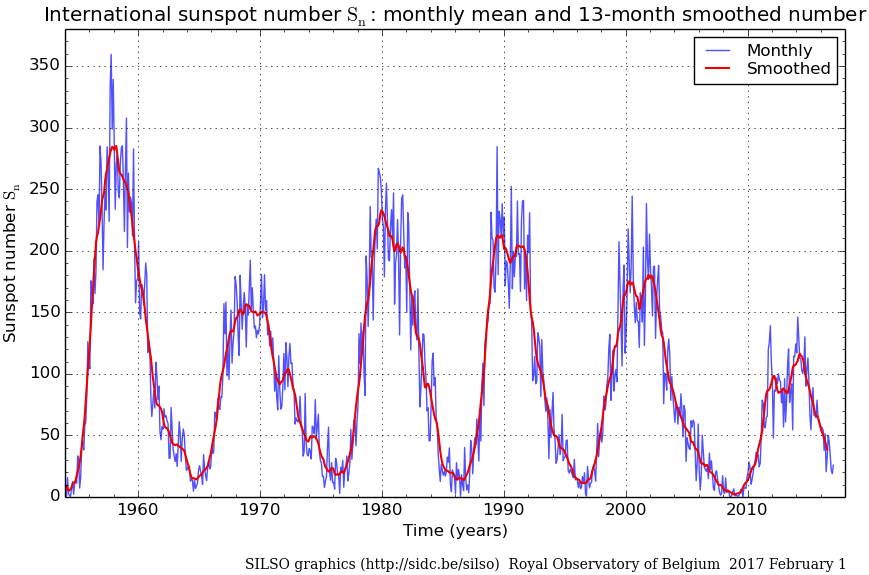
\includegraphics[width=0.6\textwidth]{images/ROB_ssn_wolfmms.png}
	}{
		\caption{Monthly mean sunspot number (blue) and 13-month smoothed monthly sunspot number (red) since 1954. Credit: \href{http://sidc.be/silso/monthlyssnplot}{SILSO data/image, Royal Observatory of Belgium, Brussels}, 2017. Update this figure before printing!!!}
		\label{fig:ROB_ssn_wolfmms}
	}
\end{figure}
%SIDC/SILSO permission request: permission not required
%image from:	http://sidc.be/silso/
The SSN observations show large variations in cycle length (9--14~years) and cycle amplitude, with peak SSNs in the range 0--300, \citep{Hathaway2015}. There also exist long-term variations, such as the 70"~year Maunder~Minimum, during which from 1645 on almost no sunspots were observed, \citep{Maunder1890}. The source of the variations in the solar cycle periods and amplitudes are variations in the meridional circulation, because their fluctuations are larger than those found in the differential rotation and in the convective motions \citep{Hathaway2015}.

%%% SSN prediction
As the SSN is commonly used as an indicator for solar activity, there exists interest in its prediction for the course of the actual and upcoming solar cycles. The continuing prediction of an already commenced activity cycle is reliable, but then the prediction of a cycle before it began is more difficult. Though, there are indications that the polar magnetic field strength during the preceding activity minimum is correlated to the strenght of the next solar cycle \citep{Schatten1987}. However, \citet{Hathaway2016} suggest that the predictability of solar cycles is generally limited -- accumulated uncertainty produced by stochastic motions in the convection zone makes predicitons further than the next solar cycle very unreliable.


\section{Heliospheric magnetic field}
\label{sec:heliospheric_magnetic_field}
%%% MBPs to canopy
In the quiet Sun during solar cycle minimum, open coronal regions are the photospheric sources of the heliospheric magnetic field (HMF). Bright points between the granules on the photosphere are detected in G-band (\SI{430}{\nano\meter}) images. They are identified as magnetic flux tubes with field strenghts of \SIrange{100}{200}{\milli\tesla} \citep{Cranmer2005}. Together these magnetic bright points (MBPs) cover around \SIrange{1}{2}{\%} of the solar surface and carry many times the flux that active regions do \citep{Sanchez_Almeida2010}. These thin flux tubes expand laterally in the low chromosphere and merge to homogeneous network fields, which expand and merge again to a large-scale canopy below the transition region (see \autoref{fig:Cranmer2005_fig1_ab}).
\begin{figure}[htb]
	\fcapside[\FBwidth]{
		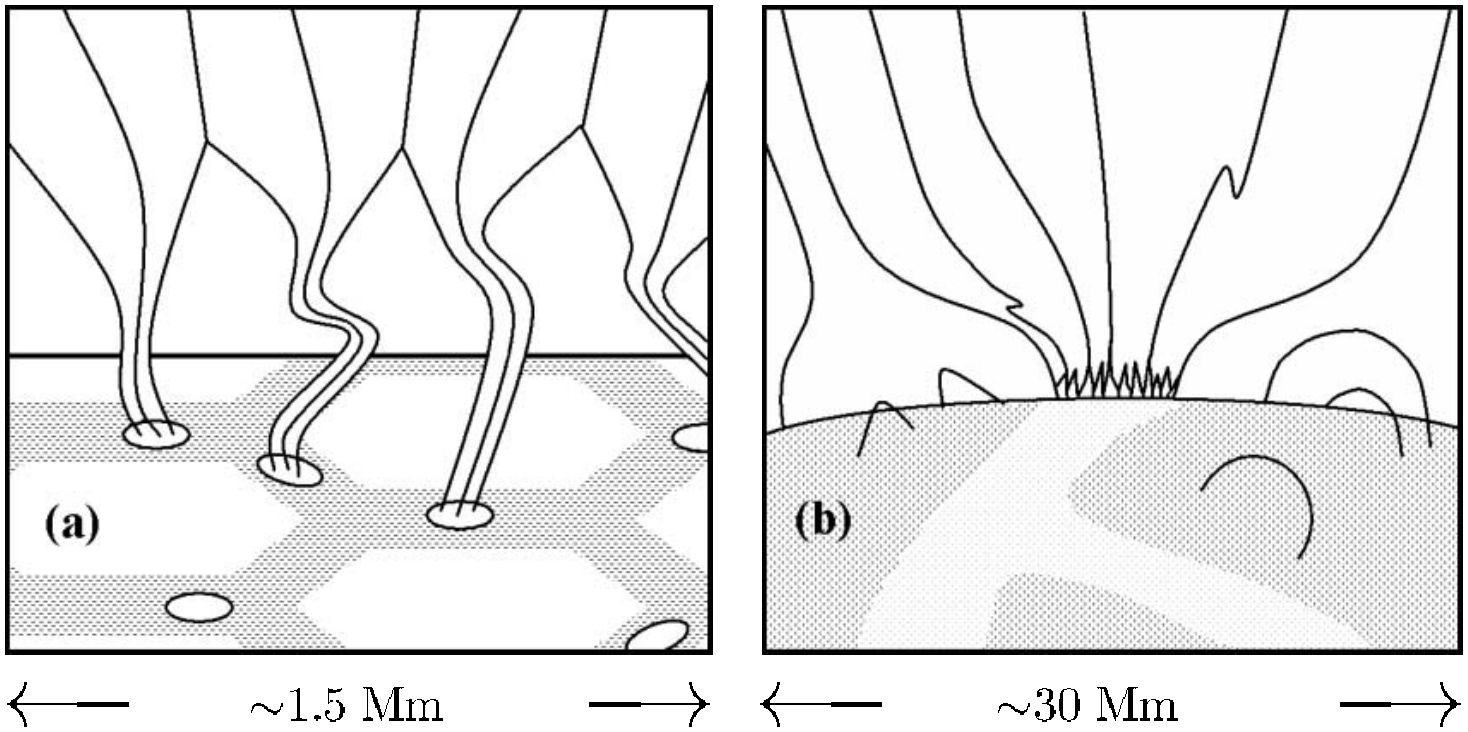
\includegraphics[width=0.6\textwidth]{images/Cranmer2005_fig1_ab.png}
	}{
		\caption{Schemata of superradially expanding magnetic flux. MBPs between granules on the photosphere are thin magnetic flux tubes that merge to a homogeneous network field (a). The network field expands again to the large-scale canopy field of the lower corona (b). Credit: \citet[][Fig.~1]{Cranmer2005}, reproduced with permission, \textcopyright~AAS.}
		\label{fig:Cranmer2005_fig1_ab}
	}
\end{figure}

%%% Alfvén waves
The MBP's convective appearance and stochastic motions result in wavelike fluctuations that propagate upward from the photosphere through the superradially expanding flux tube -- leading to incompressible waves leaking into the solar wind \citep{Cranmer2005}. These Alfvén waves propagate with a characteristic speed along the magnetic field lines -- for more details about Alfvén waves and Alfvén speed see appendix \autoref{sec:alfvén_waves}. The local Alfvén speed equals the solar wind speed at around \SI{17}{\Rs} \citep{Sittler1999,Exarhos2000}. It is believed that the solar wind is accelerated until this so-called Alfvén critical surface (cite?).\\

%%% field geometry from source surface on to heliopause
The coronal plasma expands superradially, following the magnetic field lines. However, the field strength decreases with increasing solar distance and at a distance of about \SI{2.5}{\Rs} the thermal pressure becomes larger than the magnetic pressure. Thereby the magnetic field gets frozen within the plasma and is carried by the solar wind radially outwards into the heliosphere. The distance from which the solar wind propagation uncouples from the magnetic field lines is called the source surface \citep{Schatten1969} and the thermal to magnetic pressure ratio is called plasma beta -- for more details see appendix \autoref{sec:plasma_beta}. The magnetic field changes from superradial expansion below the source surface to a radial configuration above it, this field geometry is also visible in the total eclipse image \autoref{fig:Tse2008_500_mo1}.

%%% HCS
Under solar cycle minimum conditions, a heliospheric current sheet (HCS) separates the two different magnetic polarities originating from both polar coronal holes. The HCS is roughly located in the equatorial plane, dividing both hemispheres. The analytical solar magnetic field model for solar minimum conditions, constructed by \citet{Banaszkiewicz1998}, shows this field geometry as seen in \autoref{fig:Banaszkiewicz1998_DQCS_model_raw}. The quadrupole part of their dipole plus quadrupole plus current sheet (DQCS) model considers the closed equatorial fields and allows equatorial outflows along the current sheet.
\begin{figure}[htb]
	\begin{floatrow}
		\ffigbox{
			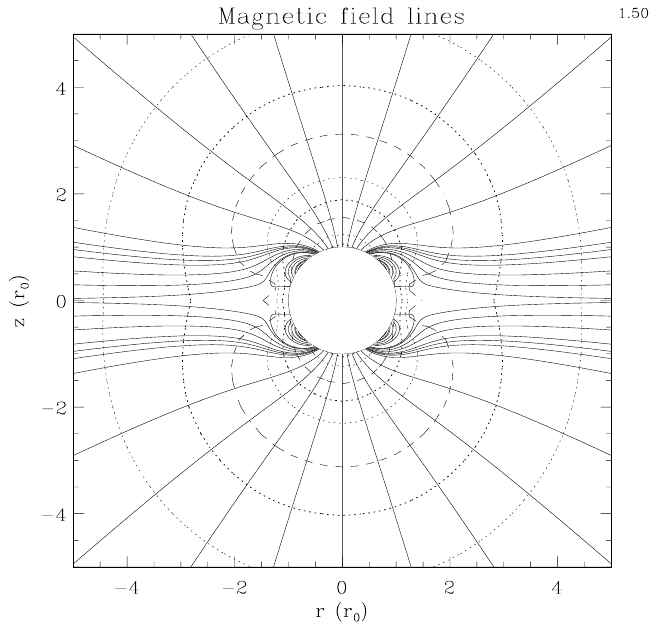
\includegraphics[width=0.45\textwidth]{images/Banaszkiewicz1998_DQCS_model_raw.png}
		}{
			\caption{Model of the solar magnetic field geometry in the polar plane for solar cycle minimum. Magnetic field lines (solid) and constant field strength surfaces (dashed) from the DQCS model are plotted. The field line spacing does not represent the field strength but provides better detail where needed. The HCS forms a few solar radii distance at $z = 0$. Credit: \citet[][Fig.~3]{Banaszkiewicz1998}, reproduced with permission, \textcopyright~ESO.}
			\label{fig:Banaszkiewicz1998_DQCS_model_raw}
		}
		\ffigbox{
			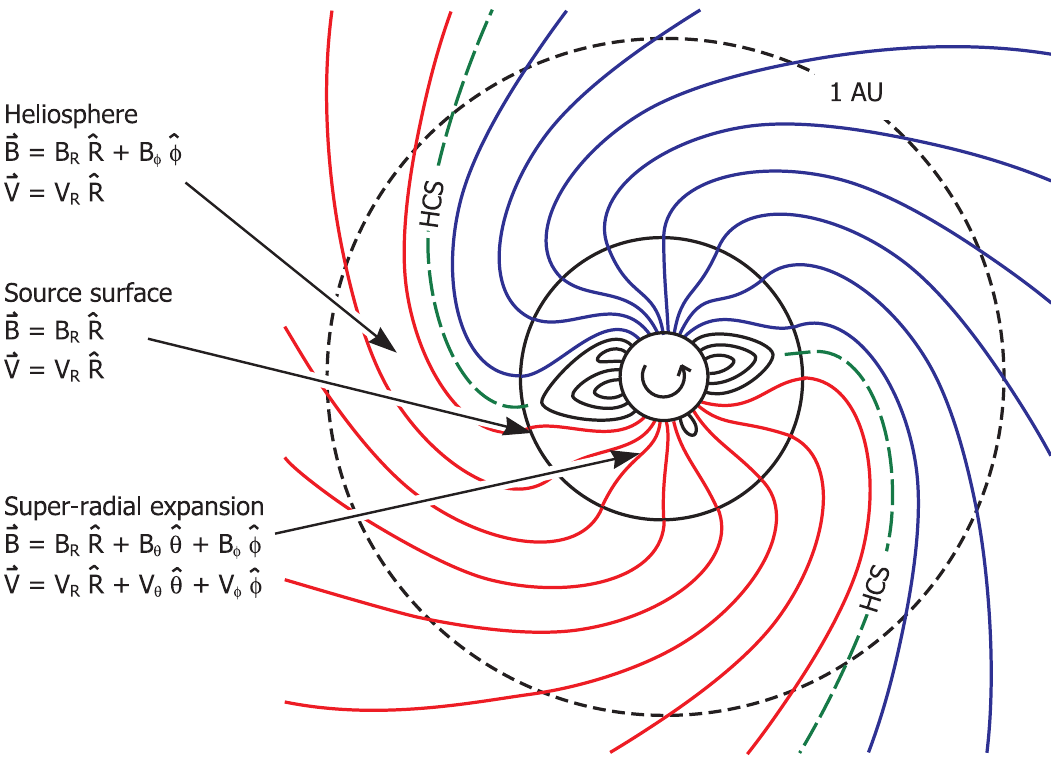
\includegraphics[width=\Xhsize]{images/Owens2013_PFSS_Sectors_screenshot.png}
		}{
			\caption{Illustration of the Parker spiral formation in the ecliptic plane outside the source surface. The HCS (green) forms between solar-wind flows of opposite magnetic field polarity (red/blue). Credit: \citet[Fig.~1]{Owens2013}, adapted from \citet[Fig.~1]{Schatten1969}, licensed under \href{https://creativecommons.org/licenses/by-nc/3.0/de/}{CC BY-NC 3.0 DE}.}
			\label{fig:Owens2013_PFSS_Sectors_screenshot}
			%Owens2013 figure permission request: open access article
		}
	\end{floatrow}
\end{figure}

%%% Parker spiral
The solar-wind source surface rotates with the Sun and thus shears the HMF into an Archimedean spiral pattern, adding an azimuthal component to the radial HMF. This geometry was anticipated by \citet{Parker1958} and is today called Parker spiral. Commonly the HCS looks more like a ballerina skirt, due to magnetic field variations, and thus the Parker spiral has sectors of different magnetic polarity, whose boundaries are separated by the HCSs. \autoref{fig:Owens2013_PFSS_Sectors_screenshot} shows the Parker spiral viewed in the ecliptic plane, where the solar rotation axis tilt of up to \SI{7.25}{\degree} leads to a slight diving into both hemispheres of opposite polarity.

%%% out to heliopause
That way the HMF is carried out to the termination shock by the solar wind. MHD simulations, based on Voyager~1 and 2 measurements within the heliosheath, provide indications about the outer structure of the heliosheath. After the termination shock, the magnetic sector boundaries are compressed and they reconnect, forming magnetic bubbles \citep{Opher2011}. These bubbles -- unconnected to the HMF -- flow away to the heliosheath tail region. Even beyond the termination shock, the solar wind plasma is confined and collimated by the twisted solar magnetic field and driven into a northern and a southern jet \citep{Opher2015}. Hence, the Sun's magnetosphere has likely a croissant-like shape with two turbulent tail-lobes, where eventually the solar wind and the HMF are mixed into the interstellar medium.


\section{Solar wind}
\label{sec:solar_wind}
%%% sw history
It is observed that cometary tails lag a few degrees from the radial direction away from the Sun, sometimes they also show fluctuations and become kinked. As such behavior could not be explained by interaction with sunlight pressure, eventually \citet{Biermann1951} concluded that cometary ion tails are influenced by a continuous flow of particles from the Sun.	%Kivelson1995, p14+91
\citet{Parker1958} considered the consequences of Biermann's conclusions and built a solar-wind model, adopting an expanding isothermal solar atmosphere. Parker also incorporated the implications for the solar magnetic field in his model and hence he laid the theoretical foundations for a continuous supersonic radial outflow of magnetized plasma. Thus, the existence of the solar wind was postulated before the first satellites measured it in~situ in 1959 \citep{Gringauz1960,Neugebauer1966}. Since that time, spacecraft are able to measure the solar wind almost continuously with in~situ magnetometer and plasma instruments (see \autoref{chap:data}). Pronounced solar-wind structures, such as CMEs and streamers, become visible with the use of space-based coronagraph imagers. From Earth, the outflow of near-Sun solar wind can also be observed during solar eclipses, see the eclipse photo in \autoref{fig:Tse2008_500_mo1}.

%%% plasma composition, parameter ranges and properties
The solar wind is a magnetized plasma consisting of electrons and ions. The ions are mainly composed of hydrogen, a small percentage of helium, and traces of oxygen, carbon, and other metals. The average abundance of helium (alphas) is about \SI{4.5}{\%} and in slow wind at solar cycle minimum conditions less than \SI{2}{\%} \citep{Feldman1978,Schwenn1983,Kasper2012}.
The solar wind is commonly approximated by an ideal incompressible magnetohydrodynamic plasma (viscosity $\mu = 0$ and electrical conductivity $\sigma = \infty$) and can be viewed as a neutral plasma. Also, its helium share is often viewed as being constant, in this case the proton density determines both the helium and electron densities. This work adopts these assumptions and treats the solar wind throughout as a proton plasma.

The properties of solar wind are highly variable in time and space. The properties are determined by the values of the solar-wind parameters magnetic field strength, proton velocity, density, and temperature. Their average magnitudes scale with solar activity, heliographic latitude, and solar distance. At a solar distance of Earth however, most of the time the parameter's typical values lie in the ranges \SIrange{3}{8}{\nano\tesla}, \SIrange{300}{500}{\km\per\s}, \SIrange{2}{8}{\per\cm\cubed}, and \SIrange{e4}{e5}{\K} (\citet[p.~92]{Kivelson1995}; \citet{Venzmer2017}). The low density of solar wind can be illustrated with a short comparison: 1~liter of air at standard pressure, expanded to a typical solar wind density of \SI{6.5}{\per\cm\cubed}, would occupy a volume of a cube with edge length of about \SI{155}{\km}.
% sw density considerations:\\
% 1 mol approx 24.7895 l/mol at 25 °C and 1 bar
% Avogadro constant N_A = 6.022140857(74)e23 mol−1
% 1 liter air @ 1 bar equates to 1/24.7895 mol = 2.4293e+22
% 2.4293e+22 / 6.5 cm-3 = 3.7374e+21 cm3 = 3.7374e6 km3 = (155 km)3
% 1 liter air @ 1 bar (need 24 ms for passing 1 dm2 area @ 15 km/h)\\
% equals\\
% 3.7e6 km3 = (155 km)3 solar wind @ 6.5 cm-3 (need 43900 a for passing 1 dm2 area @ 400 km/s)\\
Solar-wind quantities, such as particle flux densities, mass flux and plasma beta can be derived from the four listed parameters. Having the parameters in the aforementioned ranges, the solar wind is a plasma with a beta mostly greater than unity (for more on plasma beta see appendix \ref{sec:plasma_beta}).
% mean beta: 1.714\\	%from mean paper values
% low beta: 0.180\\	%from ranges above
% high beta: 8.444\\	%from ranges above

The solar wind is structured by its different sources in the solar corona. It consists of continuous streams, variable flows, and CME events. Their highly variable velocities result in compressed or rarefied regions at their interfaces. The solar wind is further structured by the magnetic field, which the plasma carries from its source region. Changes in its field direction and embedded magnetic structures influence the plasma.\\


prepare following subsections:\\
slow/fast wind\\
-> following event/structure types\\
special events/configurations, which can appear (CIRs, HCS/HPS, etc.)\\
HSS, sector boundaries, CIRs, CMEs\\

prepare next subsection:\\
different source regions: sunspots/active regions, coronal holes, and filaments.\\


SEPs, neutral atoms...\\

MHD waves (Alfvén waves)\\
in HSSs (cite?)\\
Alfvén velocity ca. 40~km/s (Kivelson1995)\\
Alfvén velocity 56.8~km/s (Veselovsky2009)\\

sonic and Alfvénic critical point positions (see Sittler \& Guhathakurta (1999))\\
sonic point and slow solar wind origin (Sheeley et al. 1997)\\


\subsection{Slow and fast streams}
%%% fast and slow solar wind
It is observed that the continuous solar wind comes in streams roughly focused at two major velocity ranges \citep{Neugebauer1966,Schwenn1983}, slow and fast streams with \SIrange{250}{450}{\km\per\s} and \SIrange{450}{800}{\km\per\s} respectively. Both types possess differences in their typical characteristics and ion compositions. Apart from its higher speeds, fast solar wind has most prominently lower proton densities ($\sim$~\SI{3}{\per\cm\cubed}) and higher temperatures ($\sim$~\SI{2e5}{\K}) than the slow solar wind, which has higher densities ($\sim$~\SI{10}{\per\cm\cubed}) and lower temperatures ($\sim$~\SI{4e4}{\K}) \citep{Schwenn1990}. The fast solar wind has a nature of coming in steady high-speed streams (HSSs) with a unique magnetic field polarity, whereas slow solar wind is much more variable in all its properties except its velocity \citep{Bame1977}.

%sources of fast wind
First soft X-ray observations of the corona, made during sounding rocket flights, showed clearly that the fast solar wind emerges from extended areas of reduced X-ray emission, subsequently called coronal holes (CHs) \citep{Krieger1973,Hundhausen1977}. The magnetic field polarities found in CHs are associated with the magnetic field directions observed in HSSs, see \autoref{fig:Hundhausen1977_fig10}.
\begin{figure}[htb]
	\fcapside[\FBwidth]{
		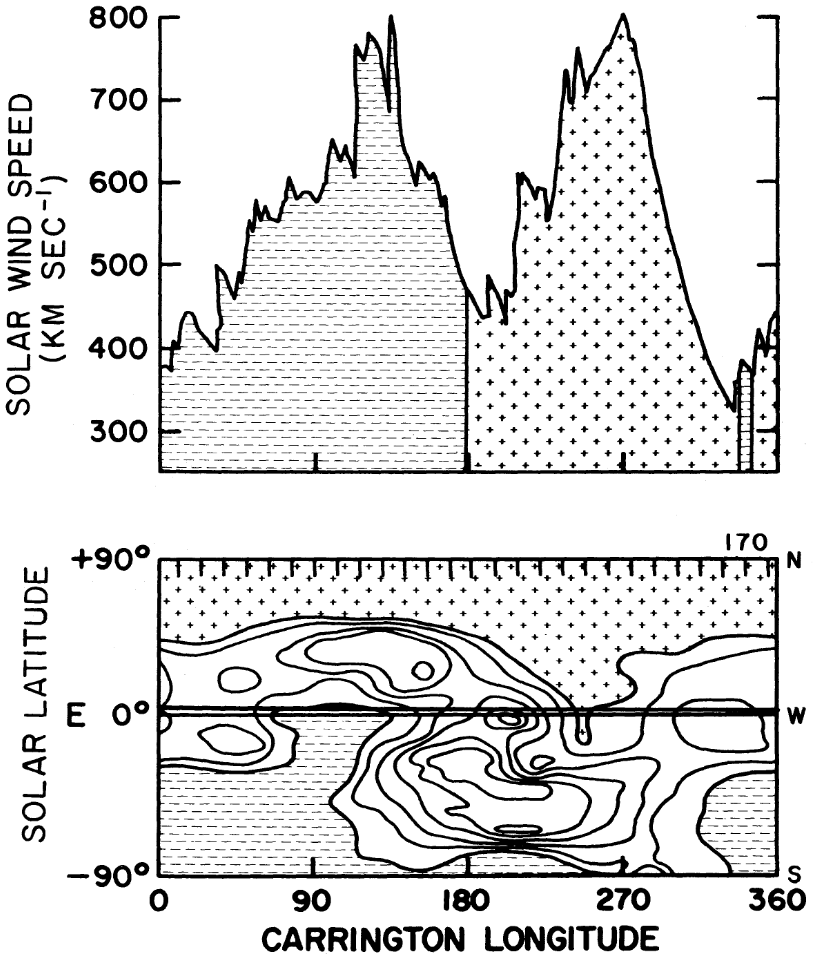
\includegraphics[width=0.5\textwidth]{images/Hundhausen1977_fig10.png}
	}{
		\caption{Solar-wind velocity with respect to its estimated source longitude (top) and coronal brightness contour map at \SI{0.5}{\Rs} above the photosphere (bottom) for the Carrington rotation 1616. The velocity is based on IMP spacecraft data, back-extrapolated to \SI{20}{\Rs}. Brightness values below a fixed threshold are shaded ($+$/$-$) corresponding to the magnetic field polarity of the underlying photosphere. The map is based on observations from the K-coronameter at the Manua~Loa Observatory. Credit: \citet[Fig.~10]{Hundhausen1977}, get permission...}
		\label{fig:Hundhausen1977_fig10}
	}
\end{figure}
In coronal regions with closed magnetic field lines the plasma is trapped, though in CHs it can escape following the open magnetic field lines outwards into space. Wave-particle interactions heat and accelerate the ions in CHs, leading to the emission of a fast solar wind \citep{Hollweg2002}. Superradial expansion of the magnetic field lines in the corona has an influence on the wind speed, actually the expansion factor is anticorrelated with the final wind velocity \citep{Wang1990}. As the field expansion is larger near the border of CHs, faster wind emerges from the mid regions of CHs, forming into HSSs. However, there are indications that the slow and fast solar wind are not only generated at different sources but from distinct mechanisms \citep{McGregor2011b}.

%sources of slow solar wind
The high variability in the slow solar wind points to the existence of different types of slow wind flows, originating from separate coronal locations and mechanisms \citep{Schwenn1983}. It is still under debate if the variability is produced by the formation mechanism of the slow solar wind or if the variability is caused during the slow solar wind's acceleration phase and further propagation \citep{Sanchez-Diaz2016}. Still, at least a part of its variability can be attributed to the interactions between slow and fast solar wind, which result in a general reduction in velocity differences and thus let solar winds of different speeds (having different properties as well) converge to a common speed regime \citep{Sanchez-Diaz2016}. Studies using remote white-light tracing of coronal material and in-situ measurements of solar wind suggest that multiple sources of slow solar wind flows exist \citep{Wang2000,Kilpua2016}. To the best of my knowledge the generally considered sources are listed in the following:
\begin{itemize*}
	\item Small CHs, because their plasma outflow is slower due to the high superradial expansion of its open field lines.
	\item CH boundaries, where the plasma is slow, due to superradial expansion as well.
	\item CH boundaries, when trapped plasma is released by reconnection between open and closed field lines.
	\item Helmet/pseudo-streamers in active regions, where transient plasma blobs are released from the cusps of closed field loops. This slow and dense material is associated with the heliospheric plasma sheet belt.
	\item Edges of active regions, which have hot plasma outflows with a single mangetic polarity \citep{Kojima1999}.
	\item The jets originating from coronal bright points might contribute to the slow solar wind \citep{Subramanian2010}.
	\item Slow CMEs can be a source of slow wind as well.
\end{itemize*}
% Kilpua2016 generally suggested sources:\\
% - CH boundaries, the plasma is slow due to superradial expansion of open field lines\\
% - transient plasma blobs that are released from the helmet/pseudo-streamers\\
% - plasma released by reconnection between open and closed field lines at the coronal hole boundaries\\
% - hot outflows with speeds up to ∼100~km/s from the edges of active regions, first reported by Kojima1999\\
% - jets originating from coronal bright points\\

It is found to be difficult to use in-situ measurements for tracing the slow solar-wind flow types to different origins and distinguishing between them, because most properties are highly variable in time \citep{Kilpua2016}. However, some indicators show tendencies to differentiate between the slow winds from different source regions. Some notable indicators are elemental ion ratios, heavy ion charge states, and the specific entropy.

The elemental composition of the coronal plasma varies with height/location in the solar atmosphere, therefore the solar wind's elemental ion ratios (e.g., $\text{He}/\text{H}$, $\text{Fe}/\text{O}$) are used to determine the origin.
The charge states of coronal heavy ions depend on the local temperature. However, the density of the outwards expanding plasma decreases fast, preventing further ionization/recombination. The charge states decouple from the local temperature and freeze in still close to the Sun. Thus, heavy ion charge ratios (e.g., $\text{C}^{+6}\!/\text{C}^{+4}$, $\text{O}^{+7}\!/\text{O}^{+6}$) in the solar wind track the coronal source temperature and especially the $\text{C}^{+6}\!/\text{C}^{+4}$ ratio is sensitive to the solar wind type \citep{Landi2012}.
At solar minimum the specific proton entropy is found to correlate with the $\text{O}^{+7}\!/\text{O}^{+6}$ ratio and thus able to trace slow solar wind sources \citep{Pagel2004}.\\
%specific entropy: $\ln\left(T_\text{p}/n_\text{p}^{\gamma - 1}\right)$ ($\gamma = 1.5$)

%solar activity dependence
The Sun's ordered dipole structure during solar cycle minima leads to polar regions with open magnetic fields, constituting large coronal holes, and to a large equatorial belt region with closed magnetic fields -- this state is clearly visible in Figures~\ref{fig:Tse2008_500_mo1} and \ref{fig:Banaszkiewicz1998_DQCS_model_raw}. This results in exclusively fast solar wind coming from the poles and higher latitudes. Whereas active regions form an equatorial streamer belt around the Sun, emitting slow solar wind. This structure was confirmed from solar-wind speed measurements done by the Ulysses spacecraft, which flew in an out-of-ecliptic solar orbit and whose mission covered a duration of more than one solar cycle \citep{McComas200809}, see \autoref{fig:McComas2008_Ulysses_orbit}.
\begin{figure}[htb]
	\centering
	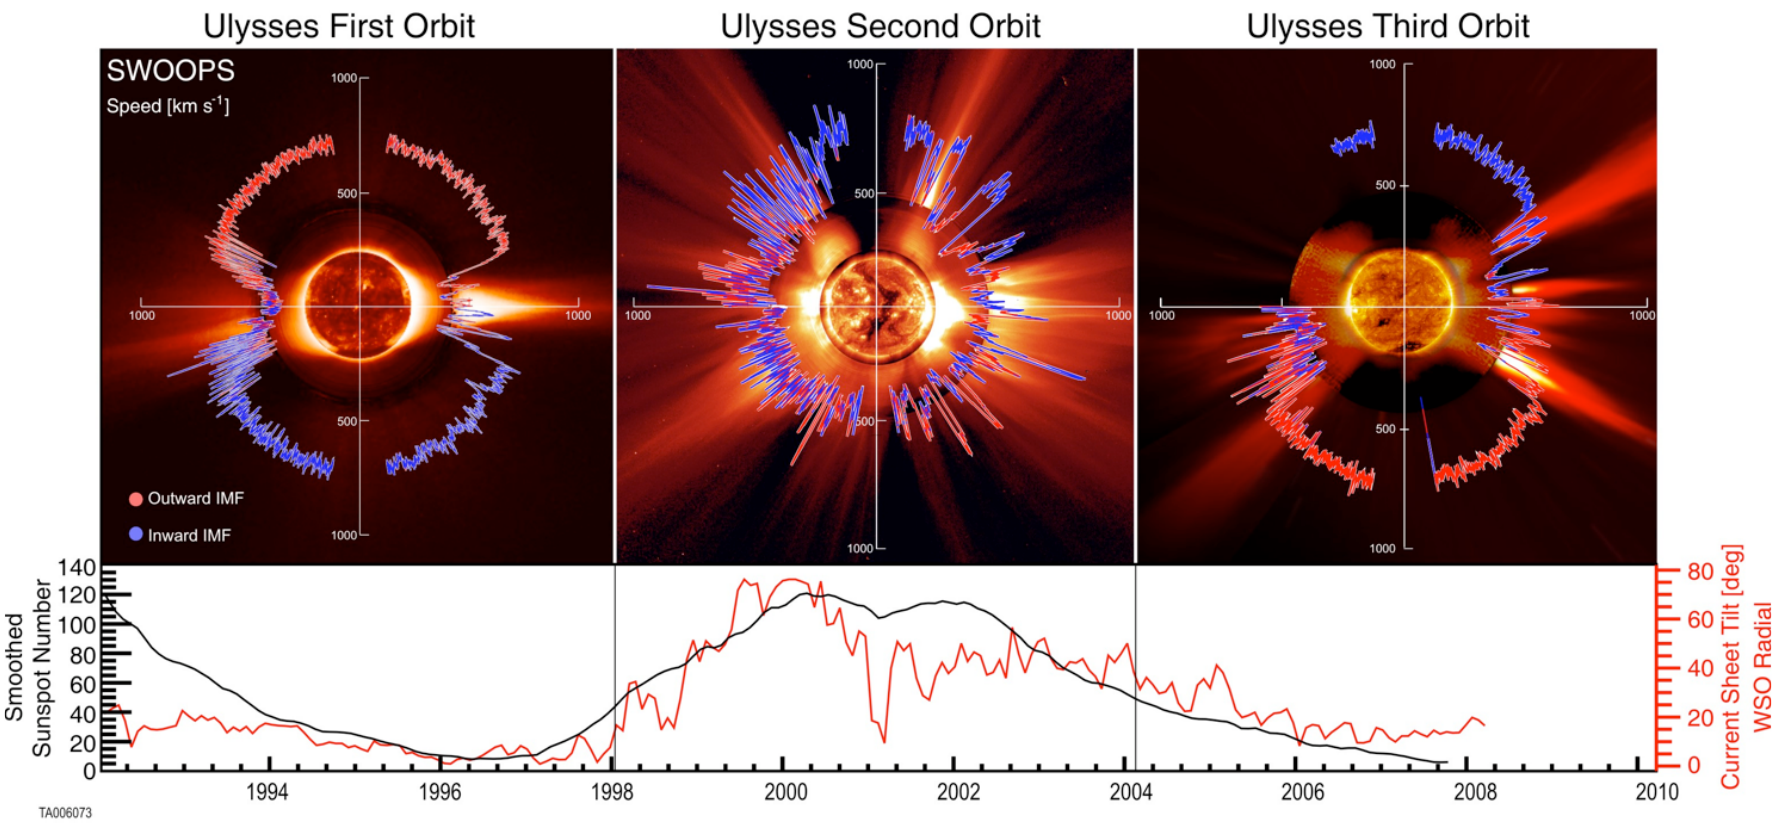
\includegraphics[width=\textwidth]{images/McComas2008_Ulysses_orbit_.png}
	\caption{Solar-wind velocity and magnetic field polarity (red/blue) with respect to heliographic latitude for the three orbits of the Ulysses spacecraft during low and high solar activity (upper panels). The data starts left and couterclockwise. The corresponding smoothed SSN (black) and HCS tilt angle (red) are plotted beneath. The background consists of solar images for solar cycle~22 minimum (1996-08-17), solar cycle~23 maximum (2000-07-12), and solar cycle~23 minimum (2006-03-28). The solar disk, inner corona, and outer corona images are from SOHO/EIT (Fe~XII at \SI{1950}{\nano\meter}), Mauna~Loa K~coronameter (\SIrange{700}{950}{\nano\meter}), and SOHO/C2 white light coronagraph. Credit: \citet[][Fig.~1]{McComas200809}, reproduced with permission, \textcopyright~American Geophysical Union.}
	\label{fig:McComas2008_Ulysses_orbit}
\end{figure}
%figure source: http://onlinelibrary.wiley.com/doi/10.1029/2003GL017136/full
%McComas200809: (a–c) Polar plots of the solar-wind speed, colored by IMF polarity for Ulysses' three polar orbits colored to indicate measured magnetic polarity. In each, the earliest times are on the left (nine o'clock position) and progress around counterclockwise. (d) Contemporaneous values for the smoothed sunspot number (black) and heliospheric current sheet tilt (red), lined up to match Figures 1a–1c. In Figures 1a–1c, the solar-wind speed is plotted over characteristic solar images for solar minimum for cycle 22 (8/17/96), solar maximum for cycle 23 (12/07/00), and solar minimum for cycle 23 (03/28/06). From the center out, we blend images from the Solar and Heliospheric Observatory (SOHO) Extreme ultraviolet Imaging Telescope (Fe XII at 1950 nm), the Mauna Loa K coronameter (700–950 nm), and the SOHO C2 white light coronagraph.
The transition of the solar magnetic field during cycle maxima induces the chaotic appearance of closed magnetic fields at higher latitudes and even at the poles. Further, coronal holes begin to invade parts of the equatorial region, this leads to recurring phases of HSSs in the ecliptic.
The alternating streams of different velocity and magnetic polarity result in interaction regions and magnetic sector boundaries.\\

The solar-wind stream pattern varies strongly with solar activity.\\

origin from closed magnetic structures in the solar corona, such as intermittent reconnection at the top of helmet streamers and from coronal hole boundaries \citep{Kilpua2016}\\

the overlapping ranges of the slow and fast solar wind \citep{McGregor2011a}\\


\subsection{Heliospheric current sheet}

% heliospheric current sheet
The heliospheric current sheet (HCS) is the separating surface between both magnetic polarities. During solar minimum the dipole axis is near the rotation axis -> the HCS is near the ecliptic.\\
During the field transition at solar maximum, the dipole axis rotates to lower latitudes, crossing the equator, and eventually ending up as a reversed dipole \citep{Jones2003}.\\




see \citet{Balogh2009}, p.~89:\\
The surface separating the two polarities is the Heliospheric Current Sheet (HCS), the largest recognisable plasma boundary\\

%ecliptic
the dipole generates magnetic sector structure in the ecliptic first identified by Ness and Wilcox (1965)\\
In most cases, there are two or four magnetic sectors in each solar rotation.\\

in maximum: the dominant (towards and away) polarities are separated by a HCS that is very complex in shape and reaches to high, near-polar heliolatitudes.\\
the position of the HCS which corresponds to the extension of the coronal neutral line into the heliosphere.\\
The HCS appears as a wavy “ballerina skirt” at around solar minimum (Thomas and Smith 1981; Jokipii and Thomas 1981), but has a very much more complex shape near solar maximum.\\
Ulysses results are compatible with a single, topologically connected HCS at least in the inner heliosphere even around solar maximum (Jones et al. 2003).\\
the HCS remains a single connected structure throughout the heliosphere even if largely inclined to the solar equator. In fact, there is evidence that at the time of magnetic reversal near solar maximum activity, the HCS rotates, in a first approximation, as the rigid equatorial plane of the solar dipole while the axis rotates from one pole to the other.\\
the HCS remains an identifiable boundary between the two dominant polarities even at the highest latitudes, through the magnetic reversal process. There is, therefore, a magnetic neutral line that reaches to high heliolatitudes in the corona.\\


%in situ observations
% sector boundaries
``Low He/H values are in particular reported near solar wind sector boundaries.'' (Borrini et al., 1981)\\
Borrini et al. (1981) had found significant depletions in $n_\alpha/n_\text{p}$ around magnetic sector boundaries which are normally imbedded in slow solar wind.\\

HCS in-situ plot?\\

equatorial ballerina model\\


\citet{Owens2013} HCSs:\\
the two polarities of the dipole being separated by the warped heliospheric current sheet (HCS), shown as the green dashed line in Figure 1.\\
As noted above the large-scale regions of opposite HMF polarity are separated by the heliospheric current sheet (HCS). Near solar minimum, the HCS encircles the Sun close to the rotational equator and hence lies close to the ecliptic plane. Thus, spacecraft in near-Earth space will generally be close in heliolatitude to the HCS and will sample HMF polarities from both polar coronal holes as the Sun rotates.\\
For a purely dipolar magnetic field typically with at least a small tilt to the rotation axis, a two-sector structure would be expected in the ecliptic plane, as sketched in Figure 1. As the quadrupolar component of the field increases, a more complex sector structure should be observed.\\
Periods of both two- and four-sector structures are seen. As the HCS is formed by open solar flux (OSF) of opposite polarities coming into contact by the non-radial expansion of separate coronal holes, the HCS maps to helmet streamers and is typically located within slow solar wind.\\


% heliospheric plasma sheet
heliospheric plasma sheet (HPS)\\

Crooker2004:\\
definition: the HPS is a high-density region containing a magnetic polarity reversal associated with the passage of the HCS.\\

Winterhalter1994 The heliospheric plasma sheet:\\
the narrow heliospheric current sheet (ca. \SIrange{3000}{10000}{\km} thick), together with the heliospheric plasma sheet in which it is embedded. The heliospheric plasma sheet region is identified by a significantly enhanced plasma beta caused by density enhancements and diminished magnetic field strength and is about 20 to 30 times the thickness of the current sheet.\\

The particularly low specific entropy structure in the slow solar wind is the high-density and low-temperature heliospheric plasma sheet (HPS). Kilpua2016\\



\subsection{Stream interaction regions}

see \citet{Balogh2009}, p.~94:\\

% interaction regions
Corotating interaction regions (CIRs)\\
Stream interaction regions (SIRs)\\
in-situ measurements (example in-situ CIR/HSS plot)\\

Streams of fast wind catch slow wind\\
-> compressions, shocks, deflections\\

formation of stream interface and stream deflection, see \autoref{fig:Owens2013_CIR_2panel_screenshot}\\
%A sketch of a stream interaction region. Left: Looking down on the ecliptic plane. Magnetic field lines within fast (slow) wind, shown in red (blue), become aligned with the stream interface by the reverse (forward) wave. Right: a view from Earth. The magnetic axis, M, and therefore the wind speed belts, are inclined to the rotation axis, R. The point in the heliosphere at which fast wind is able to catch up to the slow wind ahead of it is the stream interface (SI), which forms a spiral front in the heliosphere, shown as the black-outlined curved surface. In the frame of reference of the SI, both fast and slow wind flow toward the SI. Fast (slow) wind, shown by the red (blue) arrow, is slowed (accelerated) and deflected along the SI in the direction counter to (along) solar rotation. Right panel adapted from Pizzo (1991).
\begin{figure}[htb]
	%\centering
	\fcapside[\FBwidth]{
		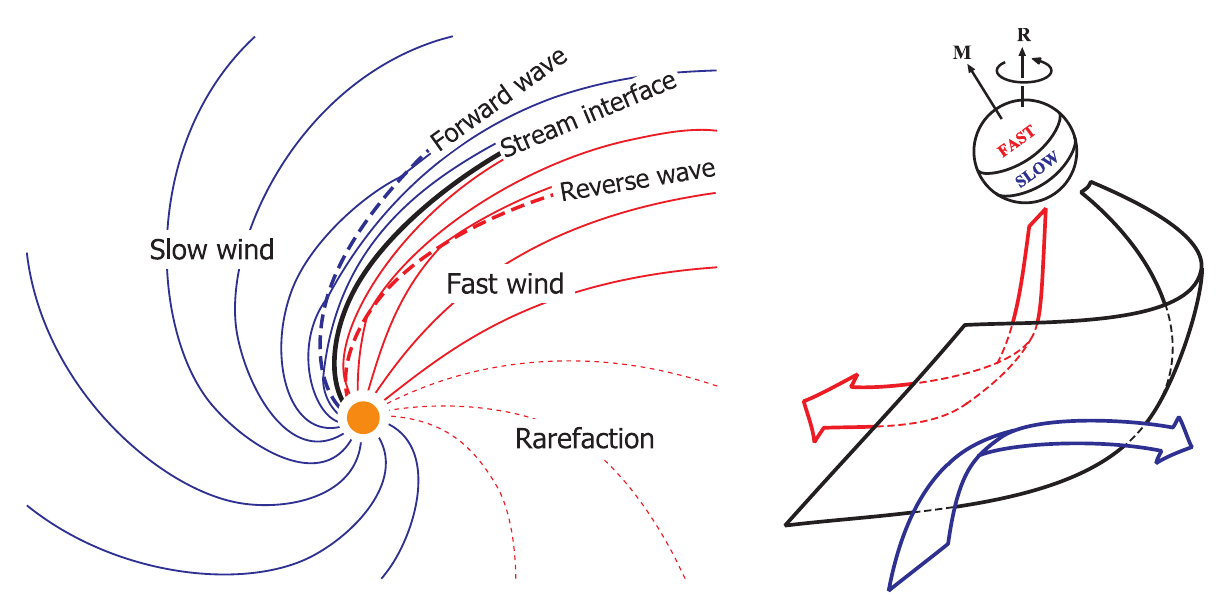
\includegraphics[width=0.6\textwidth]{images/Owens2013_CIR_2panel_screenshot.png}
	}{
		\caption{Schema of the formation of a stream interface (left) and deflection of streams (right), both generated from interactions between slow and fast solar wind. Credit: \citet[Fig.~7]{Owens2013}; right panel adapted from \citet[Fig.~2]{Pizzo1991}, licensed under \href{https://creativecommons.org/licenses/by-nc/3.0/de/}{CC BY-NC 3.0 DE}.}
		\label{fig:Owens2013_CIR_2panel_screenshot}
	}
\end{figure}
%Owens2013 figure permission request: open access article

recurrent -- with a 27-day interval\\

A multitude of structures appear in the solar wind. A period of solar wind, measured in~situ by the ACE spacecraft at the first Lagrange point 
(L1), is plotted in \autoref{fig:ACE_64s_v7_thesis_CIRs_2013-5-1_65_plot}.\\
\begin{figure}[htb]
	\centering
	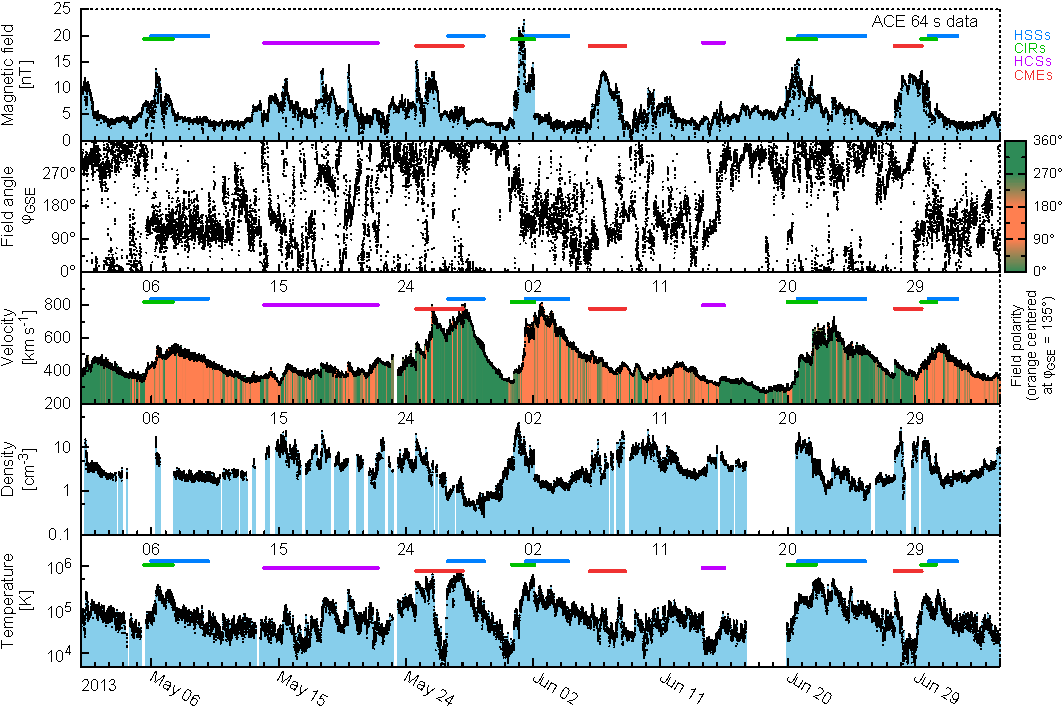
\includegraphics[width=\textwidth]{images/gnuplots/ACE_64s_v7_thesis_CIRs_2013-5-1_65_plot.pdf}
	\caption{Solar wind with several structures, measured at L1 during the time period 1~May to 5~June in 2013. The parameters are the magnetic field strength, its field angle in the ecliptic in GSE~coordinates, the proton velocity, density, and temperature. Periods of prominent solar wind structures are marked with color bars: HSSs in blue, CIRs in green, HCSs in purple, and CMEs in red. In the velocity panel also the field polarity is color coded -- assuming a Parker spiral angle of \SI{135}{\degree} at L1. Blank periods indicate bad or missing data. The data were measured with the MAG and SWEPAM instruments onboard the ACE spacecraft and are obtained from the ACE~Science~Center web interface\protect\footnotemark.}
	\label{fig:ACE_64s_v7_thesis_CIRs_2013-5-1_65_plot}
\end{figure}
\footnotetext{ACE Science Center website: \url{http://www.srl.caltech.edu/ACE/ASC/}}
MAG and SWEPAM 64-second Averaged IMF and Solar Wind Ion Parameters\\
acknowledgements to MAG/SWEPAM Team...\\

Recurrent HSSs of the same field polarity but changing peak velocity exist in this period (e.g., beginning on 6~May, 2~June, and 29~June). They are preceded by CIRs containing sector boundaries. CMEs passed on 7?~June, XXX... The 7?~June CME is displayed in higher details in \autoref{fig:ACE_64s_v7_thesis_CME_2013-6-26_6_plot}.\\
In this plot the general solar wind tendencies can be seen: the temperature scales with the velocity; compressed regions enhance the magnetic field and the density; sector boundaries/HCSs and MCs come with enhanced densities and low temperatures; MCs in CMEs have high magnetic fields and low temperatures...\\


their interactions lead to phenomena such as stream interaction regions which may persist for many solar rotations ("co-rotating" interaction regions) if the coronal source regions are quasi-stationary \citep{Balogh1999}.\\



\citet{Owens2013} SIRs:\\
Inclination of the solar magnetic axis to the solar rotation axis, as well as warps in the streamer belt, combined with the rotation of solar wind sources with the Sun, results in fast and slow solar wind successively entering the heliosphere at a fixed longitude in heliospheric coordinates, as shown in Figure 7. In such instances, fast wind (red) will catch up with slow wind ahead of it (blue) and the stream interface (SI) will take the form of a spiral front (black). The region of solar wind compression and deflection is referred to as the stream interaction region (SIR). In the quasi-steady state regime, SIRs will corotate with the Sun, and are thus referred to as corotating interaction regions (CIRs, Smith and Wolfe, 1976; Pizzo, 1991; Gosling and Pizzo, 1999; Crooker et al., 1999). In near-Earth space, CIRs are most commonly observed during the declining phase of the solar cycle, when there is typically a quasi-stable dipolar corona with significantly inclination to the rotational axis.\\
The forward and reverse waves, shown as blue and red vertical lines, respectively, have steepened into shock fronts, which typically occurs at heliocentric distances larger than 2 AU (Smith and Wolfe, 1976). Within the interaction region, bounded by the red and blue lines, the magnetic field intensity and plasma density are enhanced by compression.\\
...inclination of the stream interface means solar wind flow is systematically deflected along the SI, with fast (slow) solar wind deflected in the direction counter to (along) the solar rotation direction and poleward (equatorward) with respect to the heliographic equator.\\
As a consequence of the relationship between the HCS and the coronal streamer belt, the HCS is located at the centre of the slow solar wind band near the Sun. Indeed, the HCS is often observed to be embedded within SIRs and CIRs (Gosling and Pizzo, 1999). As the forward wave/shock propagates into the slow solar wind ahead of a CIR it can eventually overtake the HCS boundary, making it more likely for the HCS to be embedded within a CIR with increasing distance from the Sun (Thomas and Smith, 1981).\\

As the CIRs move outward, they coalesce into larger scale, merged structures (the so-called Merged Interaction Regions, or MIRs) from about 10 AU or so (Burlaga1985).\\


\subsection{Coronal mass ejections}
\label{sec:coronal_mass_ejections}
%%% CMEs and MCs

Corona observations, made by the first space-based coronagraph located on Skylab in 1973/74, show...\\

Embedded in the solar-wind streams are CMEs. Their frequency in near \SI{1}{\au} measurements varies between almost zero during solar cycle minima up to a daily rate of about $0.5$ during times of solar maximum (Richardson \& Cane 2012).\\


CMEs (link to previous coronagraph image; in situ CME/MC plot)\\

flares + CMEs\\

% reconnections
The solar differential rotation wraps the magnetic field lines, accumulating tension, leading eventually to relief with a magnetic reconfiguration by field line reconnections.\\
--> release of much energy --> flares, CMEs\\


Coronal mass ejections (CMEs) (discovery (Carrington), definition (Hundthausen?), models, GCS (conception of 3-dim CME shape --> enables Earth arrival time forecast from modeled direction and velocity))\\

active regions:\\
sunspots, magnetic reconnections, flares, post-eruptive arcades\\

coronagraph figure of CME (COR2 image, SECCHI/STEREO), see \autoref{fig:CME_COR2_0120923_182400_dbc2A}\\
\begin{figure}[htb]
	\fcapside[\FBwidth]{
		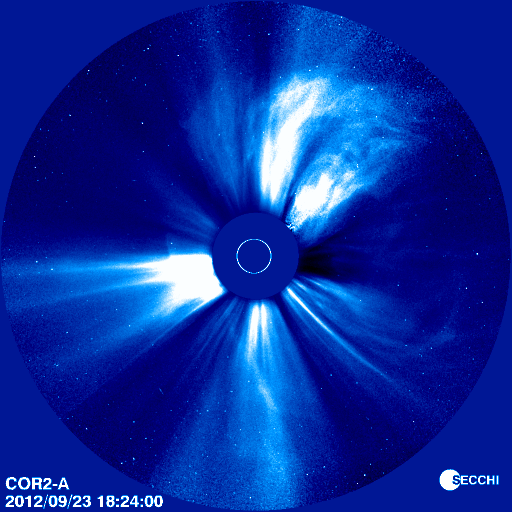
\includegraphics[width=0.5\textwidth]{images/CME_COR2_0120923_182400_dbc2A.png}
	}{
		\caption{Coronagraph image of a CME. STEREO~A, SECCHI-A COR2, COR2-A, date 20120923-182400. Credit: NASA/STEREO... find optimal event...}
		\label{fig:CME_COR2_0120923_182400_dbc2A}
	}
\end{figure}

in-situ solar wind figure of same CME (recent one from 2016)\\

CME-plasma properties\\
+ flares and SEPs often accompany CMEs\\

magnetic clouds (MCs)\\
See BS magnetic cloud model in analyses methods chapter
MVA...\\

CME with MC, solar wind in-situ measurements and impact on the magnetosphere (Kp), see \autoref{fig:ACE_64s_v7_thesis_CME_2013-6-26_6_plot}\\
\begin{figure}[htb]
	\centering
	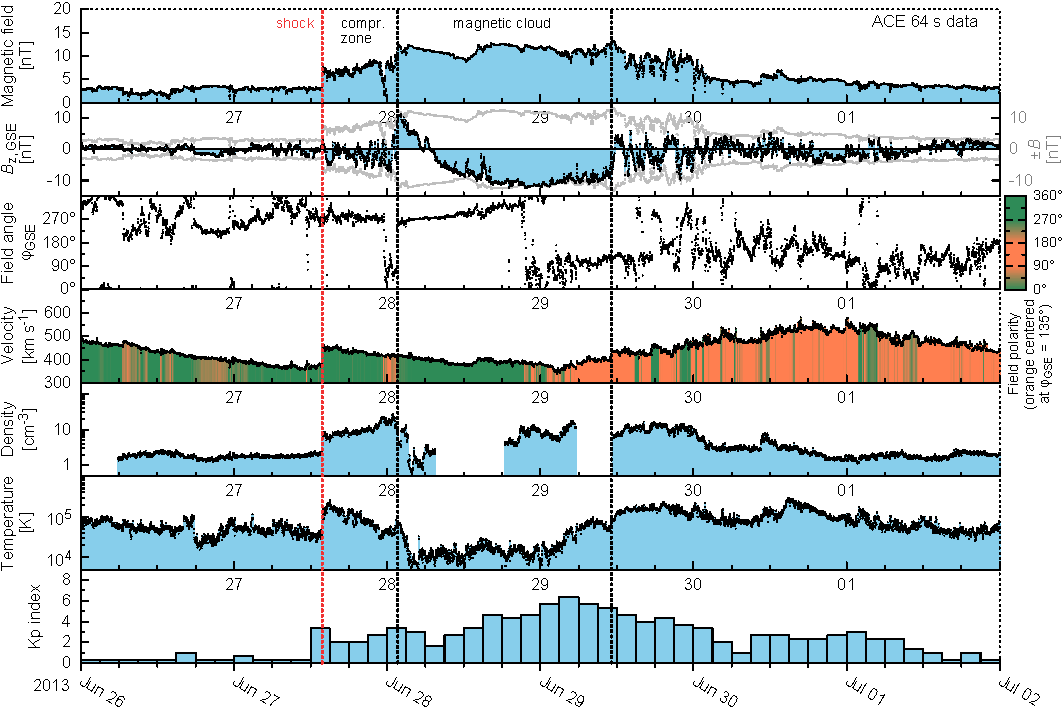
\includegraphics[width=\textwidth]{images/gnuplots/ACE_64s_v7_thesis_CME_2013-6-26_6_plot.pdf}
	\caption{Solar wind with a CME, measured at L1 during the time period 26~June to 2~July in 2013. The parameters are the magnetic field strength, its z-component and ecliptic field angle in GSE~coordinates, the proton velocity, density, temperature, and the \Kp-index. In the velocity panel also the field polarity is color coded -- assuming a Parker spiral angle of \SI{-45}{\degree}. The shock, the compression zone, and the duration of the magnetic cloud are indicated by dotted lines. Blank periods indicate bad or missing data. The solar wind data was measured with the MAG and SWEPAM instruments onboard the ACE spacecraft and is obtained from the ACE~Science~Center. The \Kp{} data is obtained from the GFZ~Potsdam.}
	\label{fig:ACE_64s_v7_thesis_CME_2013-6-26_6_plot}
\end{figure}

%%%%%%%%%%%%%%%%


history (paper); properties -> CHs and streamers; fast/slow; Ulysses -> SIRs; in situ fig -> CMEs; coronagraph fig; in situ fig\\

%++dynamics and magnetic field++\\
%rotating nebula to solar rotation\\
%rotation + convective motion -> differential rotation (first discovered by sunspot observations; helioseismology -> inner rotation, tachocline)\\
% meridional flow -> 22 year cycle || convective cells\\
% 22y convection cycle + magnetic field -> 11ys solar cycle (magnetic field activity cycle, polarity change, sunspot number)\\
keywords:\\
SSN -> poloidal/toroidal field -> magnetic surface activity (butterfly diagram) -> min/max polar CHs (quiet/active Sun figure) -> HMF (quiet B-field figure) -> quiet HMF Parker spiral (figure) -> solar wind -> slow/fast sw pattern (Ulysses figure)\\



\section{Space weather}
\label{sec:space_weather}

Solar wind influences the terrestrial magnetosphere and can disturb sensitive technical systems\\
understanding its properties helps with prediction of events\\

various space weather effects, for instance disturbances in magnetic fields, aurorae, episodes of enhanced radiation, atmospheric losses and stripping of cometary tails. figures of these effects?\\

influences on human infrastructure/technical systems/animals (such as birds and whales -> Vanselow2017 10.1017/S147355041700026X)\\

reference to \citet{Bothmer2007}, maybe images\\

\subsection{Solar influence on Earth}
\label{sec:solar_influence_on_earth}

solar wind's impact on Earth\\

Carrington made first connection between terrestrial magnetic field and solar flares. correct?\\

%see Bartels1962:
there are several types of solar-terrestrial relations, \citet{Bartels1962} listed:\\	%Zuordnung solarer Beobachtungen zu terrestrischen\\
a) irregular flare and CME effects (Carrington)\\
b) 11"~year solar cycle effects\\
c) 27"~day solar rotation effects\\
d) daily effects (x-ray and light)\\

seasonal effects from Earth orbital distance, inclination (solar rotation axis angle) and Earth tilt (see \autoref{fig:sun-earth_seasonal_geometry_draft})\\
\begin{figure}[htb]
	\centering
	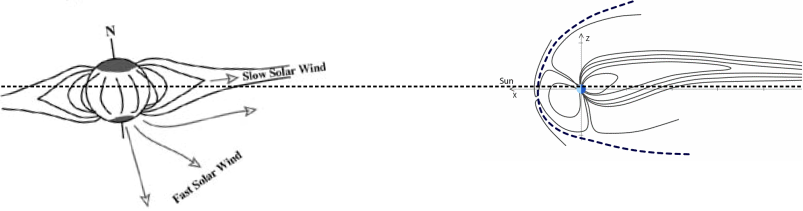
\includegraphics[width=\textwidth]{images/own_figures/sun-earth_seasonal_geometry_draft.png}
	\caption{Sun-Earth geometry in the plane orthogonal to the ecliptic (not to scale); Solar magnetic field-magnetosphere geometry. Seasonal effects are: solar tilt, Earth distance and Earth tilt. make new figure, see Hundhausen1977, p.~285...}
	\label{fig:sun-earth_seasonal_geometry_draft}
\end{figure}

solar wind and its structures\\
solar radiation\\
solar energetic particles (SEPs)\\
gravitation\\

magnetosphere\\
ionosphere?\\
aurorae\\
geomagnetic storms (several days, from CMEs)\\
substorms (few hours, from CIRs??)\\

see Akasofu2011\\

for humans and their technology important effects: enhanced radiation, geomagnetic storms\\
lovely, disruptive, dangerous consequences <-- read in VBbook\\

at Earth the solar wind total energy flux ($1.45~\text{mW/m}^2$) is only about one millionth of the solar radiation flux (see \citet[p.~153]{Schwenn1990})\\

"The principal users affected by geomagnetic storms are the electrical power grid, spacecraft operations, users of radio signals that reflect off of or pass through the ionosphere, and observers of the aurora." NOAA cite\\


\subsection{Magnetosphere}
\label{sec:magnetosphere}

The magnetosphere's shape is formed by the dynamic pressure balance. The structure is similar to the heliosphere in the ISM.\\

bow shock, magnetotail, magnetosheath, magnetopause\\
add ecliptic and terrestrial tilt angle; with plasmoid?\\
see \autoref{fig:heliosphere_image002}\\
\begin{figure}[htb]
	%\centering
	\fcapside[\FBwidth]{
		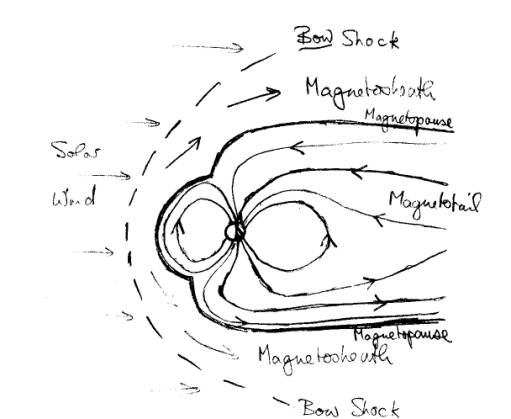
\includegraphics[width=0.5\textwidth]{images/heliosphere_image002.jpg}
	}{
		\caption{temp figure ``The cavity is called the magnetosphere. It has a relatively well-defined outer boundary, the magnetopause.''}
		\label{fig:heliosphere_image002}
	}
\end{figure}

turbulence with sw (KH or RT instabilities)\\

Earth magnetic field strength at a height of \SI{36000}{\km} (geostationary): $\approx$\SI{100}{\nT}\\
Earth magnetic field strength at the surface - equator: $\approx$\SI{30000}{\nT} - poles: $\approx$\SI{60000}{\nT} (cite?)\\

magnetopause = current layer??\\

two extreme cases of Bz orientation: parallel/antiparallel\\
compression/reconnection (see \autoref{fig:Bothmer1998book_p116_fig4_8_sw})\\
\begin{figure}[htb]
	%\centering
	\fcapside[\FBwidth]{
		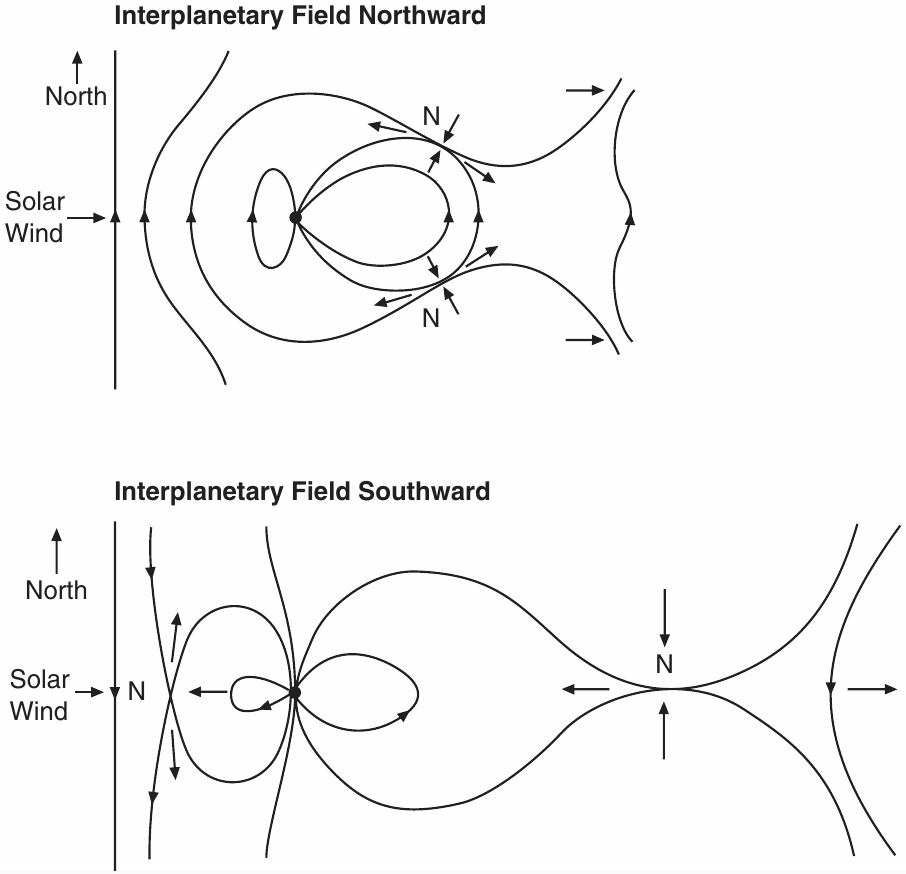
\includegraphics[width=0.5\textwidth]{images/Bothmer2007book_p116_fig4_8_sw.png}
	}{
		\caption{reconnection and compression depending on the interplanetary magnetic field orientation. Credit: \citet[p.~116, Fig.~4.8]{Bothmer2007}, adapted from Dungey1961, 1963. get permission... accelerated flows are arrowed; N points are X points...}
		\label{fig:Bothmer1998book_p116_fig4_8_sw}
	}
\end{figure}

standoff distance:	\citep[p.~112]{Bothmer2007}
\begin{align}
	d = \frac{107.4}{1 R_\text{E}} (N V^2)^{-1/6}
\end{align}

Even in ``ancient'' times (when?) a correlation between solar particles and disturbances in the magnetosphere were known of (Bartels1962).\\

magnetosphere variations due to solar wind\\
magnetosphere protects from radiation (maybe from solar wind stripping atmosphere away?)\\

effects: aurorae, ...\\

ring current systems\\

definition of:\\
magnetic storm...\\
substorm...\\

subsection Ionosphere?\\
its variations due to solar radiation (day/night cycle and flares)\\
ionosphere -> TEC -> GNSS error\\


Solar wind interaction processes with the magnetosphere:\\
there are several underlying physical mechanisms, whose contribution is not yet quantified'?'\\
physical mechanisms:\\
- reconnection\\
- compression\\
- turbulence\\
- induction?\\

three ways for solar wind momentum and energy transfer into magnetosphere:\\
- sw entering sphere\\
- waves/eddies\\
- reconnection\\


\subsection{Solar wind--magnetosphere coupling}
%\label{sec:solar_wind_magnetosphere_coupling}

E-field produced by solar wind:	%VBth p124
acts on magnetospheric plasma\\
\begin{align}
	\textbf{E}_\text{IMF} = -\textbf{V} \times \textbf{B}_\text{IMF}
\end{align}
from Lorentz force F = -e vxB\\
E = -F/e\\
Because of high plasma conductivity the E-field is not existent.\\

Axford1964 viscous interaction (of turbulent nature, KH/RT instabilities, KH instabilities at the flanks of the magnetosphere) is a viable source of drag force/solar storm energy input into magnetosphere\\

Otto\&Nykyri1982 KH instabilities/vortices force magnetic reconnection even at northern IMF and are able to account for observed mass flux\\

\citet{Newell2007} and \citet{Newell2008}: coupling consists of merging and viscous part (reconnection and turbulence)\\
merging part: universal sw-magnetosphere coupling function; rate magnetic flux is opened at the magnetopause ($d\Phi_\text{MP}/dt$)\\
viscous part: reconnection due to Kelvin-Helmholtz instabilies at the boundary ($n^{1/2} v^2$)\\
equation for the least variance linear prediction of Kp: $Kp = 0.05 + \num{2.244e-4} d\Phi_\text{MP}/dt + \num{2.844e-6} n^{1/2} v^2$\\
combination of both terms works best (r = 0.866)\\

Merkin2013 MHD simulation of velocity shear at magnetosphere boundary with northern IMF; KH instabilities; double-vortex sheet structure\\

% mass flux considerations:\\
% mass per second per Earth disc...\\
% R_E = 6371.008 km\\
% A_E = pi * R_E² = 127516438.219 km²\\
% m_p = 1.672621898e-27 kg\\
% v = 400 km/s\\
% n = 6.5 cm-3 = 6.5e15 km-3\\
% mass flux = m_p * n * v * A_E = 0.0013863641126 kg/s/A_E\\
% = 1.4 g/s/A_E = 5 kg/h = 120 kg/d/A_E = 44 t/a/A_E\\

% Wikipedia: https://en.wikipedia.org/wiki/Solar_wind
% The wind exerts a pressure at 1 AU typically in the range of 1–6 nPa (1–6×10−9 N/m2), although it can readily vary outside that range.
% The ram pressure is a function of wind speed and density. The formula is
% P = mp * n * V2= 1.6726×10−6 * n * V2
% where mp is the proton mass, pressure P is in nPa (nanopascals), n is the density in particles/cm3 and V is the speed in km/s of the solar wind.[citation needed]


\subsection{Geomagnetic indices}
\label{sec:geomagnetic_indices}
Geomagnetic observatories are distributed widely over the globe, measuring the local magnetic field at their position. Several sets of stations, covering specific regions, are defined to monitor the state of different parts of the magnetospheric system. Magnetic measurements from these sets define several geomagnetic indices. The International Association of Geomagnetism and Aeronomy (IAGA) supports the following global geomagnetic indices which are serviced by the International Service of Geomagnetic Indices (ISGI)\footnote{ISGI website: \url{http://isgi.unistra.fr/}}:
The $aa$~index is designed to represent the amplitude of the global geomagnetic activity, normalized to a geomagnetic latitude of \SI{+-50}{\degree}. The $am$~index characterizes the global geomagnetic activity. The \Kp{}~index is designed to measure geomagnetic disturbances from solar particle radiation [reword...]. The \Kp~index is described in more detail in \autoref{sec:kp_index}. The $Dst$~index monitors the intensity of the magnetospheric ring current. The $PC$~index monitors the polar cap magnetic activity -- it approximates the amount of energy which entered the magnetosphere through solar-wind coupling. The $AE$~index and its relatives $AU$, $AL$ and $AO$ measure the magnetic effects of the northern auroral electrojet.
The first three listed indices (\textit{aa}, \textit{am} and \Kp{}) are calculated from different sets of local 3"~hourly $K$~indices, which measure the local magnetic disturbances at the observatories. There exist several more indices that are based on some of those listed above.\\

[for \Kp{}, $AA$ and $Dst$ read Section 7.4 in book \citet{Bothmer2007}...\\
$Dst$ (read book Jursa1985 p. 4-31)]\\

\citet{Lockwood2014} even used geomagnetic indices to reconstruct the near-Earth solar wind magnetic field strength and velocity back to 1845.\\



%%%%--  next chapter  --%%%%

\chapter{Instrumentation and data sources}
\label{chap:data}
%COFI -- chapter outline and flow integration

%\section{Instruments}
%\label{sec:instruments}

For analyzing the solar wind and related effects on the Sun there are remote instruments (solar imager and coronagraphs) and in-situ instruments (magnetometer and plasma detector).\\
Here the basic principles of the latter are described, because the analyses performed in this thesis are based on in-situ solar-wind measurements.\\


%\section{Data sources}

Different kind of data are used for the investigations in this thesis -- collected from observatories at various locations.\\

Spacecraft / data sets\\

Positions:\\
Earth:\\
	imager, magnetosphere\\
L1 - first Lagrangian point:\\
	ACE (siehe auch space weather spacecraft Liste)\\
	Wind etc. (OMNI)\\
	DSCOVR\\
1~au orbit\\
	STEREO~A and B\\
inner heliosphere:\\
	Helios~1 and 2\\
	PSP\\
outer heliosphere:\\
	Voyager~1 and 2\\
	Ulysses\\

A time coverage overview of the data sets used in the analyses of this thesis (SSN, \Kp~index, LRO, HRO, Helios~1 and 2) is plotted in \autoref{fig:timeline_SSN_with_data_and_sc}.\\
\begin{figure}[htb]
	\centering
	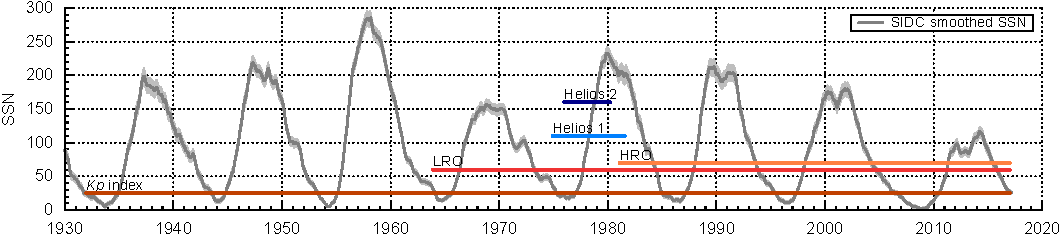
\includegraphics[width=\textwidth]{images/gnuplots/timeline_SSN_with_data_and_sc.pdf}
	\caption{Time coverage of the \Kp~index, low and high resolution OMNI, Helios~1 and Helios~2 data sets until end of 2016. The SIDC 13-month smoothed monthly SSN is plotted in the background. add cycle number...}
	\label{fig:timeline_SSN_with_data_and_sc}
\end{figure}


\section{Magnetometer}
%\label{sec:magnetometer}

Spacecraft nowadays carry two different magnetometer types, one for measuring the magnetic field direction and its strength and the other for observing the magnetic flux and detecting waves.\\

A flux gate magnetometer consists of two coils around a core -- one coil with alternating current, wich is compared with the induced current signal from the other. Without external magnetic field both patterns match. The core is easier magnetized in direction of an existing external magnetic field, in which case the patterns differ. It measures...\\
In a search coil magnetometer one coil is placed around a core; measures plasma waves - where?\\

Because these magnetometer types are directional, they often are placed in two sets of triaxial configurations, attached on booms to minimize the influence of the spacecraft's own magnetic field.\\
L-> which is generated by surface charges?/electrons?/ionization?/the instruments?\\
%https://en.wikipedia.org/wiki/Spacecraft_magnetometer

examples:\\
ACE/MAG -- fluxgate magnetometer\\


\section{Plasma detector}
%\label{sec:plasma_detector}

several spectrometers with different energy ranges\\

isotope spectrometer - isotopic abundances of SEPs\\
ionic charge analyzer - charge state of SEPs\\
sw ion mass spectrometer - \\
sw ion composition spectrometer - \\
radio burst tracker\\


A plasma detector measures the ion energy frequency distribution, which consists basically only of protons and alphas in solar wind (see \autoref{fig:ion_energy_spectrum_plot}). see also \autoref{sec:solar_wind}
\\
\begin{figure}[htb]
	%\centering
	\fcapside[\FBwidth]{
		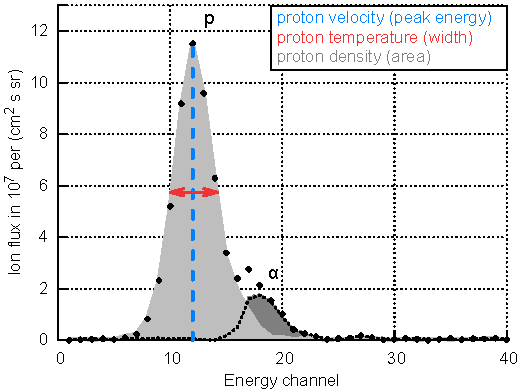
\includegraphics[width=0.5\textwidth]{images/gnuplots/ion_energy_spectrum_plot.pdf}
	}{
		\caption{Example of an ion energy spectrum with synthetic data. Here proton and helium (alpha) peaks are distinguishable...}
		\label{fig:ion_energy_spectrum_plot}
	}
\end{figure}
%figure adapted from source: http://www.goembel.biz/sun.html

From the energy spectrum the velocity, density and temperature can be derived.\\

The bulk velocity is derived from the distribution's average energy.\\
The number density is the area of the distribution.\\
The temperature scales with the distribution's width.\\

% source: ftp://spdf.gsfc.nasa.gov/pub/data/ulysses/plasma/swoops/ion/swoops_ion_users_guide_update_20030214.txt
% ``Plasma parameters are calculated by numerical integration of velocity-weighted
% ion distributions over a E/q range chosen to include the thermal proton and
% alpha-particle populations. Under extremely hot conditions, there can
% sometimes be some overlap between these populations. Additionally, during
% periods when the solar-wind temperature is exceptionally low the experiment can
% not properly measure the temperature. Care has been taken to estimate the
% instrument background from channels that do not contain data, and the effects
% of background have been removed from the integration. The velocity space 
% resolution of the experiment is better in the energy dimension than in the
% angular dimensions.''

ACE/SWEPAM\\	%https://sci-hub.ac/10.1023/A:1005040232597


\section{Sunspot number}
\label{sec:sunspot_number}

SSN history in section basics\\
add SSN figure of history incl. Maunder minimum?\\
SIDC/SILSO... see paper...\\
SSN Version~2.0\\
WDC-SILSO -- World Data Center-Sunspot Index and Long-term Solar Observations\\
%https://de.wikipedia.org/wiki/Sonnenfleck#Geschichte


\section{\Kp{}~index}
\label{sec:kp_index}
Julius~Bartels introduced the \textit{K}~index in 1938 and designed it to measure the intensity of geomagnetic disturbances \citep{Bartels1939}. Its name originates from 'Kennziffer' -- the german word for characteristic digit. The \textit{K}~index is a measure for the maximal variation of the surface magnetic field, observed in a magnetogram within 3"~hour intervals. Its scale in the range 0--9 is a quasi-logarithmic representation of the actual magnetic field strength's variations.

The Planetary \textit{K}~index (\Kp{}) is a planetary geomagnetic disturbance index, introduced by Bartels in 1949 at the Institute for Geophysics, University of Göttingen \citep{Bartels1949}. \Kp{} is the weighted average of 13 \textit{Ks}~indices, which are the standardized versions of the local \textit{K} indices measured at 13 observatories. These contributing observatories are located around \SI{+-50}{\degree} geomagnetic latitude and their distribution is biased towards Europe (see \autoref{fig:Kp_map}).
\begin{figure}[htb]
	%\centering
	\fcapside[\FBwidth]{
		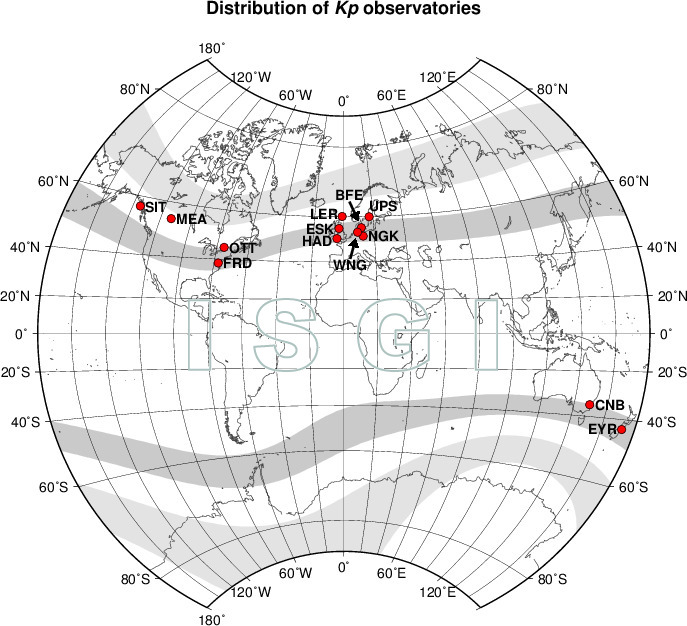
\includegraphics[width=0.6\textwidth]{images/Kp_map.jpg}
	}{
		\caption{Distribution of the 13 \Kp{} observatories. Courtesy of \href{http://isgi.unistra.fr/indices_kp.php}{International Service of Geomagnetic Indices (ISGI)}, 2013.}
		\label{fig:Kp_map}
	}
\end{figure}
% contacted via email: got permission
%\url{http://isgi.unistra.fr/indices_kp.php}

To benefit from its higher precision, its scale, in the range 0--9 as well, is further divided into thirds, represented by the suffixes '$+$', 'o' and '$-$' (e.g., 3o, $3+$, $4-$, 4o). The \Kp{}~indices are often visualized in musical diagrams, where they are stacked into periods of 27~days to enable the detection of recurrent activities, as seen in \autoref{fig:musi1612}.
\begin{figure}[htb]
	\centering
	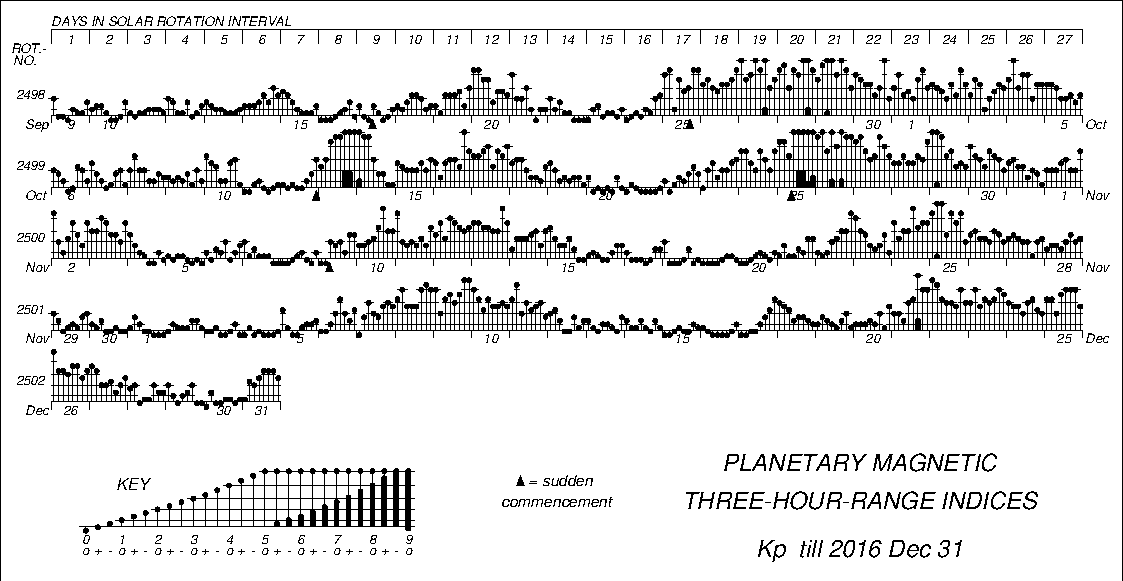
\includegraphics[width=\textwidth]{images/musi1612.pdf}
	\caption{Bartels musical \Kp{} diagram for the time period from September until end of December 2016. Two sudden commencements with following geomagnetic storms, having a maximal \Kp{} of $6+$, can be seen in October. Credit: \href{http://www.gfz-potsdam.de/en/kp-index/}{GFZ~Potsdam}, 2017, licensed under \href{https://creativecommons.org/licenses/by/4.0/}{CC BY 4.0}.}
	\label{fig:musi1612}
\end{figure}
%ftp://ftp.gfz-potsdam.de/pub/home/obs/kp-ap/music/

The \Kp{}~index can be converted to the 3"~hour equivalent $ap$~index, which represents the magnetic field strength at a surface position of about \SI{50}{\degree} dipole latitude. The conversion is done via a table defined by Bartels, in which the value of the \textit{ap}~index is scaled in units of \SI{2}{nT} (see \autoref{tab:kp_to_ap_table}).
\begin{table}
	\caption{Defined table for the conversion from the \Kp~index to the equivalent \textit{ap}~index, which represents the magnetic field strength in units of \SI{2}{nT}.}
	\label{tab:kp_to_ap_table}
	\centering
	\begin{tabular}{lssssssssssssss}
		\Kp	&0o	&0+	&1-	&1o	&1+	&2-	&2o	&2+	&3-	&3o	&3+	&4-	&4o	&4+\\
		\textit{ap}	&0	&2	&3	&4	&5	&6	&7	&9	&12	&15	&18	&22	&27	&32\\
		\hline
		\Kp	&5-	&5o	&5+	&6-	&6o	&6+	&7-	&7o	&7+	&8-	&8o	&8+	&9-	&9o\\
		\textit{ap}	&39	&48	&56	&67	&80	&94	&111	&132	&154	&179	&207	&236	&300	&400
	\end{tabular}
\end{table}
There are further geomagnetic indices which are derived from the \Kp{}~index. They include $Ap$, the daily $ap$ average, $Cp$, the daily $ap$ sum mapped via a defined table to the range \numrange{0}{2.5}, and $C9$, a mapping of $Cp$ via a defined table to the range \numrange{0}{9}. The definitions of Q"~days (quiet days) and D"~days (disturbed days) are also obtained from the \Kp{}~index.

The International Association of Geomagnetism and Aeronomy (IAGA) adopted the \Kp{}~index in 1954. The \Kp{}~index was maintained in Göttingen until January 1997 -- now the German Research Centre for Geosciences (GFZ) in Potsdam supplies the \Kp{}~index and thereof derived indices. The GFZ provides historical and quicklook data of the indices via their website\footnote{GFZ website for geomagnetic indices: \url{http://www.gfz-potsdam.de/de/kp-index/} (existent in 2017-10-29)}. The data was extended backwards and is available from 1932 onwards.\\

Several indicators/quantities are based on the \Kp{}~index:\\
The NOAA G-Scale for geomagnetic storms (G~1 to G~5) is based on the \Kp~index\footnote{NOAA Space Weather Scales website: \url{http://www.swpc.noaa.gov/noaa-scales-explanation} (existent in 2017-10-29)}.\\
The equatorward auroral boundary position correlates with the \Kp~index (cite?).\\
The variation of the total electron content (TEC) of the ionosphere correlates with the \Kp~index (cite?). The TEC has influence on global navigation satellite systems (GNSS). A part of their positional error scales directly with TEC (in extreme cases up to about \SI{30}{\m}).\\

"It is designed to measure solar particle radiation by its magnetic effects."\\

Because of the effects on sensitive technical systems, methods for \Kp{} forecasting are developed.\\
- Wing \Kp{} model (link)\\
- Potsdam quicklook data (link)\\
- Alexej \Kp{} correlation forecast model (link)\\
- In this work we derive relations for \Kp{} nowcast from in-situ solar-wind measurements and \Kp{} forecast from remote solar-wind stream/CME observations.\\

% acknowledgments:\\
% The results presented in this thesis rely on the \Kp{}~index, calculated and made available by the German Research Centre for Geosciences in Potsdam from data collected at magnetic observatories. We thank the involved national institutes, the INTERMAGNET network and ISGI (isgi.unistra.fr).\\


\section{OMNI data set}
\label{sec:omni_data_set}

see paper...\\

a data set merged from different sources\\
The OMNI data \citep{King2005} were obtained from the GSFC/SPDF OMNIWeb interface.\\

from spacecraft located near the Lagrange point L1 upstream of Earth\\
time-shifted to the bow shock of the magnetosphere\\

OMNI2 H0 MRG1HR (1963--201308)
Cite from CDAweb: Hourly near-Earth solar-wind magnetic field and plasma data, energetic proton fluxes (>~1 to >~60~MeV), and geomagnetic and solar activity indices.

NASA, Goddard Space Flight Center (GSFC), Space Physics Data Facility (SPDF): \url{http://spdf.gsfc.nasa.gov/}\\	%exintent in 2016-08-18
- Coordinated Data Analysis Web (CDAWeb): \url{http://cdaweb.gsfc.nasa.gov/}\\	%exintent in 2016-08-18
- OMNIWeb Plus: \url{http://omniweb.gsfc.nasa.gov/}\\	%exintent in 2016-08-18
%OMNIWeb Data Documentation: http://omniweb.gsfc.nasa.gov/html/ow_data.html

intercalibrated multi-spacecraft solar-wind data\\
Various spacecraft contribute to the interplanetary magnetic field (IMF) and solar-wind plasma OMNI data, as seen in \autoref{fig:timeline_OMNI_SC_IDs}.\\
\begin{figure}[htb]
	\centering
	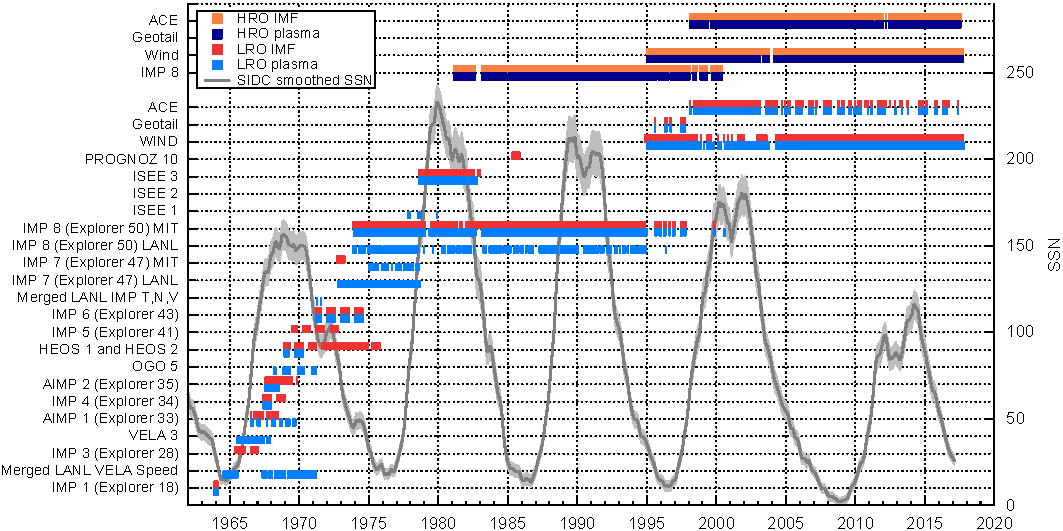
\includegraphics[width=\textwidth]{images/gnuplots/timeline_OMNI_SC_IDs.pdf}
	\caption{IMF and solar-wind plasma data source spacecraft for the high and the low resolution OMNI (HRO, LRO) data sets until end of 2016. The SIDC 13-month smoothed monthly SSN is plotted in the background. add cycle number...}
	\label{fig:timeline_OMNI_SC_IDs}
\end{figure}

\subsection{Solar Wind Structures}
Solar Wind Structures (SWS) list\\
derived by Richardson.... from OMNI data (only?)
see chapter2...\\

permission received.\\

%http://cedarweb.vsp.ucar.edu/wiki/index.php/Tools_and_Models:Solar_Wind_Structures
characterization of near-Earth solar-wind structures since 1963\\
SWS lists \citep{Richardson2000} and \citep{Richardson2012}


\section{Helios probes}
\label{sec:helios_probes}

see Helios data readme.txt\\
see paper\\

two different fluxgate magnetometers and a search coil magnetometer\\

see \autoref{fig:helios2}
\begin{figure}[htb]
	\begin{floatrow}
		\ffigbox[\FBwidth][]{
			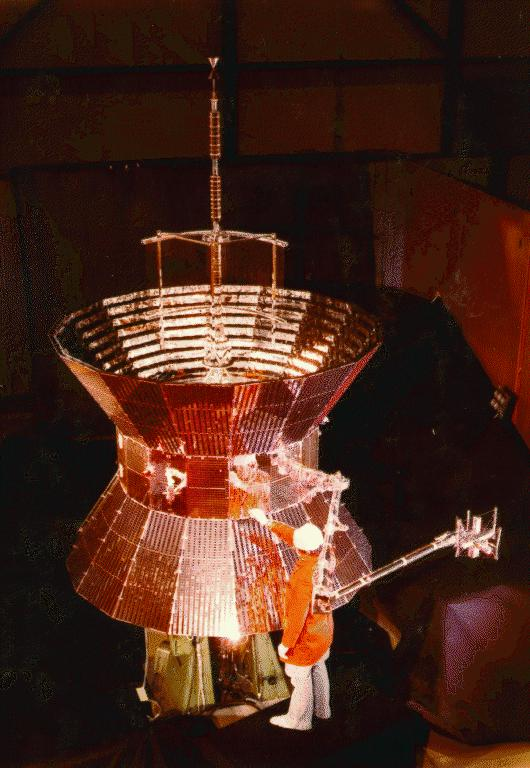
\includegraphics[width=0.3\textwidth]{images/helios2.jpg}
		}{
			\caption{One of the nearly identical twin Helios spacecraft. Credit: \href{https://solarsystem.nasa.gov/galleries/helios}{NASA/Max Planck Institute for Solar System Research}.}
			\label{fig:helios2}
			%source: https://solarsystem.nasa.gov/galleries/helios
			%NASA has no copyrights to its contents
		}
		\ffigbox[\Xhsize]{
			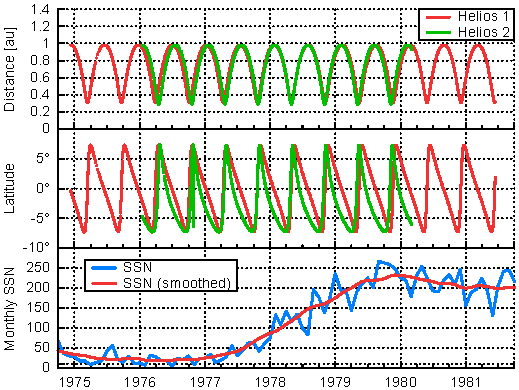
\includegraphics{images/gnuplots/Helios12_1h_r_b_ssn_plot.pdf}
		}{
			\caption{Plot of the Helios probes' solar distance and HGI latitude over their mission time, together with the monthly SSN and 13-month smoothed monthly SSN.}
			\label{fig:Helios12_1h_r_b_ssn_plot}
		}
	\end{floatrow}
\end{figure}

solar distance, HGI latitude and sunspot number during the Helios missions; see \autoref{fig:Helios12_1h_r_b_ssn_plot}\\

Helios~1 and 2 orbits in the ecliptic plane and in the latitude polar plane (see \autoref{fig:Helios12_orbits_ecliptic_polar})\\
\begin{figure}[htb]
	\centering
	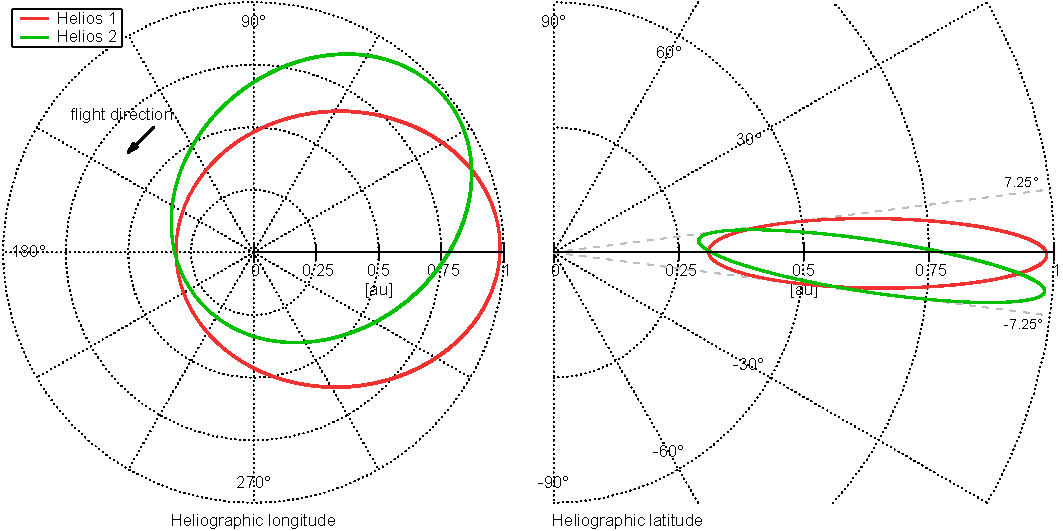
\includegraphics[width=\textwidth]{images/gnuplots/Helios12_orbits_ecliptic_polar.pdf}
	\caption{Orbits of the Helios~1 (red) and Helios~2 (green) spacecraft in the solar equatorial plane (left) and polar plane (right) (HGI-coordinates). change colors?}
	\label{fig:Helios12_orbits_ecliptic_polar}
\end{figure}

The Helios magnetic field and plasma data frequency over heliocentric distance and over heliographic latitude are plotted in \autoref{fig:helios_data_frequency}.\\
\begin{figure}[htb]
	\centering
	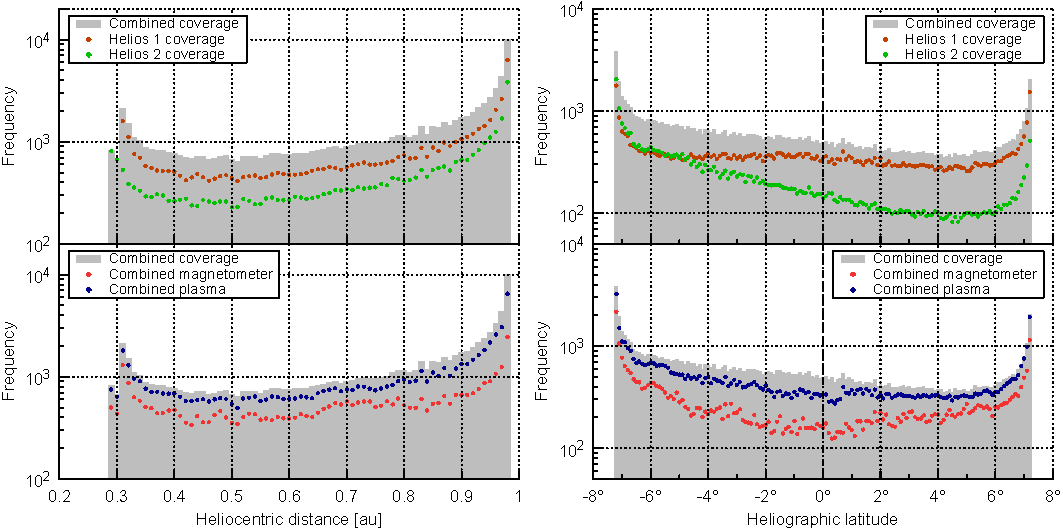
\includegraphics[width=\textwidth]{images/gnuplots/helios_data_frequency.pdf}
	\caption{Helios data frequency over heliocentric distance with bins of \SI{0.01}{au} (left panels) and over heliographic latitude with bins of \SI{0.1}{\degree} (right panels). The frequency data is based on the hourly merged magnetometer and plasma data sets for Helios~1 and Helios~2. The top panels show the frequencies for Helios~1 and Helios~2 individually and the bottom panels those for the magnetometer and plasma data. avoid white lines...}
	\label{fig:helios_data_frequency}
\end{figure}

Solar wind data courtesy of R.~Schwenn, Max-Planck-Institut für Aeronomie, Lindau, magnetic field data courtesy of F.~Neubauer, Universität zu Köln. (see paper; into acknowledgements...)\\

%see presi 1.07 Inside Helios-Origins and Evolution-Salem.ppt
%see book Schwenn1990 https://books.google.de/books?id=W1DuCAAAQBAJ&printsec=frontcover&dq=Physics+of+the+Inner+Heliosphere+I.+Large-Scale+Phenomena&hl=de&sa=X&redir_esc=y#v=onepage&q=Physics%20of%20the%20Inner%20Heliosphere%20I.%20Large-Scale%20Phenomena&f=false



data sources -- see paper for replacing the following data\\
solar-wind parameters: ACE, Helios, OMNI\\
geomagnetic indices: Kp, OMNI\\

Space Physics Data Facility (SPDF)\\

HELIOS~1 and 2 - orbital Parameters\\
\url{http://spdf.sci.gsfc.nasa.gov/pub/data/helios/helios1/traj/}\\
\url{http://spdf.sci.gsfc.nasa.gov/pub/data/helios/helios2/traj/}\\

Helios hourly merged mag \& plasma data:\\
HELIOS1\_COHO1HR\_MERGED\_MAG\_PLASMA\_2965.txt\\
HELIOS2\_COHO1HR\_MERGED\_MAG\_PLASMA\_3096.txt\\
\url{http://cdaweb.gsfc.nasa.gov}\\
temporal coverage of merged data\\
Helios 1: 1974-12-10 - 1981-06-14\\
Mag data availability: 42.6~\%\\
Plasma \& orbit data availability: 76.4~\%\\
Helios 2: 1976-01-01 - 1980-03-04\\
Mag data availability: 54.4~\%\\
Plasma \& orbit data availability: 91.8~\%\\


\section{Real-time solar-wind data}

Advanced Composition Explorer (ACE)\\
s/c figure, launch date was 25 August 1997\\

Wind, STEREO, SOHO, CELIAS\\

data errors/gaps...\\
Several services/alerts are based on the data streams from real-time measurements. (L1 alerts, etc.)\\

DSCOVR as replacement was launched on 11~Februar 2015. It is NOAA's SWPC real-time solar-wind prime source since 27 July 2016.\footnote{\url{http://www.swpc.noaa.gov/products/real-time-solar-wind}}\\
